\documentclass[11pt,a4paper]{article}
\usepackage[T1]{fontenc}
\usepackage[utf8]{inputenc}
\usepackage[margin=25mm,headheight=14pt]{geometry}
\usepackage{microtype}
\usepackage{amsmath,amsthm,mathtools}
\usepackage{newtxtext,newtxmath}
\usepackage{booktabs,array,longtable}
\usepackage{xcolor}
\usepackage{tikz}
\usetikzlibrary{arrows.meta,positioning,calc}
\usepackage{enumitem}
\usepackage{fancyhdr}
\usepackage{caption}
\usepackage{listings}
\usepackage{hyperref}
\usepackage[nameinlink,noabbrev]{cleveref}
\definecolor{inkblue}{HTML}{234A68}
\definecolor{softblue}{HTML}{F0F5F8}
\definecolor{rulegray}{HTML}{D8E0E5}
\definecolor{textgray}{HTML}{52616B}
\hypersetup{colorlinks=true,linkcolor=inkblue,citecolor=inkblue,urlcolor=inkblue,
  pdftitle={Canonical Forms Need Not Be Subgraphs},
  pdfauthor={Research draft prepared with ChatGPT},
  pdfsubject={Surreal forms, canonical subgraphs, exact graph minima,
    sparse and high-girth representations}}
\pagestyle{fancy}
\fancyhf{}
\fancyhead[L]{\small\color{textgray}Canonical forms need not be subgraphs}
\fancyhead[R]{\small\color{textgray}Research draft}
\fancyfoot[C]{\thepage}
\renewcommand{\headrulewidth}{0.3pt}
\setlength{\parskip}{3.5pt}
\setlength{\parindent}{1.2em}
\setcounter{tocdepth}{2}
\numberwithin{equation}{section}
\newtheorem{theorem}{Theorem}[section]
\newtheorem{lemma}[theorem]{Lemma}
\newtheorem{proposition}[theorem]{Proposition}
\newtheorem{corollary}[theorem]{Corollary}
\theoremstyle{definition}
\newtheorem{definition}[theorem]{Definition}
\newtheorem{example}[theorem]{Example}
\newtheorem{question}[theorem]{Question}
\theoremstyle{remark}
\newtheorem{remark}[theorem]{Remark}
\crefname{lemma}{Lemma}{Lemmas}
\crefname{corollary}{Corollary}{Corollaries}
\crefname{proposition}{Proposition}{Propositions}
\crefname{remark}{Remark}{Remarks}
\crefname{question}{Question}{Questions}
\Crefname{remark}{Remark}{Remarks}
\Crefname{question}{Question}{Questions}
\newcommand{\No}{\mathbf{No}}
\newcommand{\D}{\mathbb{D}}
\newcommand{\Z}{\mathbb{Z}}
\newcommand{\N}{\mathbb{N}}
\newcommand{\val}{\operatorname{val}}
\newcommand{\rk}{\rho}
\newcommand{\gir}{\operatorname{girth}}
\newcommand{\outdeg}{\deg^{+}}
\newcommand{\pref}{\preccurlyeq_{\!s}}
\newcommand{\cpref}{\prec_{\!s}}
\newcommand{\cut}[2]{\left\{#1\,\middle|\,#2\right\}}
\newcommand{\emptycut}{\{\,\mid\,\}}
\newcommand{\can}{C}
\newcommand{\sizeV}{\mathrm{v}}
\newcommand{\sizeE}{\mathrm{e}}
\newcommand{\code}[1]{\texttt{#1}}
\newcommand{\maxdeg}{\Delta}
\captionsetup{font=small,labelfont=bf}
\lstset{basicstyle=\small\ttfamily,columns=fullflexible,keepspaces=true,
  frame=single,rulecolor=\color{rulegray},breaklines=true,showstringspaces=false,
  xleftmargin=0.6em,xrightmargin=0.6em}
\tikzset{vertex/.style={circle,draw=inkblue,fill=white,minimum size=9mm,
  inner sep=1pt,font=\small}, edge/.style={-{Latex[length=2mm]},thick,draw=inkblue},
  elabel/.style={font=\scriptsize,fill=white,inner sep=1pt}}

\title{\color{inkblue}\LARGE\bfseries Canonical Forms Need Not Be Subgraphs\\[5pt]
\large Rigidity and sparsity of surreal option graphs:\\
two five-vertex counterexamples, sharp graph minima, minimal-form\\
enumeration, an exact girth--size tradeoff, and planar high-girth forms}
\author{Research draft prepared with ChatGPT}
\date{20 September 2026}

\begin{document}
\maketitle
\thispagestyle{empty}
\begin{abstract}
A question explicitly posed by Matthew Roughan in 2018 asks whether the
canonical representation of a surreal number is a subgraph of every other
representation of that number. We give a negative answer using a five-vertex
form of $1/2$: its underlying undirected graph is a pentagon, while the canonical
graph is a triangle. The obstruction therefore persists after all edge
directions, left/right designations, roots, and numerical labels are forgotten.
Five vertices and form rank three are both smallest possible for such a
counterexample. A second, structurally different five-vertex witness, whose
intermediate values are only $0$ and $1$, is recorded beside it; an exhaustive
search shows that there are exactly sixteen five-vertex counterexamples, of
which eight are triangle-free and four have value $1/2$.

The negative answer leads to positive structural results in two opposite
directions. On the rigid side, every finite representation contains a directed
path through all sign-prefix values of its value; for a dyadic $x$ with birthday
$b$ and reduced denominator $2^k$, the minimum vertex count, edge count, and
cycle rank are respectively $b+1$, $b+k$, and $k$; there are exactly
$2^{b(b-1)/2-k}$ vertex-minimal forms, all containing the canonical graph as a
value- and side-preserving spanning subgraph; and the canonical form is the
unique edge-minimizer. On the sparse side, every finite-birthday surreal value
has representations of arbitrarily large girth, obtained here by two independent
constructions: a spaced-spine construction with exact size, rank, and cycle-rank
formulas, and a tree-and-spine construction whose output is additionally planar
with maximum degree at most three. For the single value $1/2$ the exact
girth--size tradeoff is determined: the minimum number of vertices at girth at
least $g$ is $3$, $5$, and $g$ for $g=3$, $g=4$, and $g\geq5$, and every cycle
length except four is realized exactly. Consequently the values whose canonical
graphs occur in every representation are exactly the integers, both in the
weakest unlabelled sense and in a stronger rooted, directed, $L/R$-preserving
sense. Two disjoint transfinite results are proved at $\omega$: a limit-stage
obstruction to choosing all prefix representatives coherently, and a
triangle-free representation of $\omega$ with unchanged birthday. Exact-arithmetic
code exhausts all $3{,}860$ forms with at most five vertices and checks them with
three oracles of different kinds.
\end{abstract}

\begin{center}
\fcolorbox{rulegray}{softblue}{\begin{minipage}{0.92\linewidth}
\small\textbf{Status and scope.}
The elementary counterexamples and the general theorems below are accompanied by
complete mathematical proofs. This is an unrefereed, AI-assisted research draft,
not a claim of machine-checked formalization or independently certified
priority. A targeted literature search on the date above found the original
question and later related work, but no subsequent resolution. Search coverage
and publisher access were limited, and this absence is not a certificate of
novelty. Bibliographic metadata for the 2023 journal version of the source was
located, but its full text was not retrievable; no claim is made that the 2018
wording persists unchanged there. The result concerns dependency graphs of
\emph{forms}, not graphs obtained by identifying every pair of equal-valued
vertices.
\end{minipage}}
\end{center}

\begin{center}
\fcolorbox{rulegray}{softblue}{\begin{minipage}{0.92\linewidth}
\small\textbf{Provenance.}
This article merges two independently prepared research packages on the same
question, \code{canonical-forms-need-not-be-subgraphs} and
\code{sparse-option-graphs}. Both answered the question negatively, at the same
weakest reading, with a five-vertex form of $1/2$ whose underlying graph is a
pentagon; both used the same conventions (structurally distinct raw forms as
vertices, the reduced Dali canonical map, the dependency DAG with unique sink
$O$). The two witnesses, however, are genuinely different forms, not renamings
of one another: the first hangs its long arm on the left of the root and passes
through a vertex of value $-1$, and has form rank three; the second hangs its
long arm on the right, uses only the values $0$ and $1$, has the empty form as a
direct option of the root, and has form rank four. Both are printed in full in
\cref{sec:pentagon}. Beyond the shared pentagon the two packages diverge almost
completely: the first supplies the prefix theory, exact graph minima, the
classification and count of vertex-minimal forms and the minimality of the
counterexample; the second supplies the planar degree-three high-girth
construction, the full cycle spectrum and exact extremal function at $1/2$, the
stronger rooted-colour classification, and the high-girth form of $\omega$.
Where the two packages proved the same statement by different routes, both
proofs are retained and labelled.
\end{minipage}}
\end{center}

\clearpage
\tableofcontents
\clearpage

\section{The question and the answer}
\label{sec:intro}

The distinction between a number and a particular expression for that number
is especially important for surreal numbers. A form is a recursively specified
pair of sets of earlier forms. Several forms can have the same numerical value
while retaining different dependency graphs. This makes it natural to ask
whether a canonical representation is an unavoidable graph-theoretic core.

In the caption to Figure~3 of \emph{Surreal Birthdays and Their Arithmetic},
Roughan asks the following question explicitly \cite[p.~7]{Roughan2018}:
\begin{quote}
``is the canonical form always a subgraph of any alternative form of the same number?''
\end{quote}
The paper distinguishes identity of forms from equality of values and uses the
reduced dyadic, or Dali, canonical representation. We use precisely that
convention. The problem is a small, concrete question about representation
structure, rather than a major foundational conjecture about the surreal field.
Its advantage as a research target is that a finite counterexample can settle
the universal assertion without any numerical approximation.

The question is ambiguous about what an embedding must preserve. There are at
least three reasonable readings: actual occurrence of the canonical form as a
subform; containment with numerical and left/right labels preserved; and
containment of the underlying unlabelled undirected graph. The first implies the
second and the second the third, so refuting the weakest reading refutes all
three at once. That is what the counterexamples below do. They say nothing about
containment as a graph minor or after replacing edges by paths.

Here is the entire counterexample. The symbols on the left name \emph{forms}:
\begin{equation}
\label{eq:main-five}
 O=\emptycut,\qquad
 P=\cut{O}{},\qquad
 N=\cut{}{O},\qquad
 Z=\cut{N}{},\qquad
 F=\cut{Z}{P}.
\end{equation}
Their values, in order, are $0,1,-1,0,1/2$. The graph of $F$ consists of the two
paths
\begin{equation}
\label{eq:main-paths}
 F\longrightarrow Z\longrightarrow N\longrightarrow O,
 \qquad
 F\longrightarrow P\longrightarrow O.
\end{equation}
It is a pentagon after orientations are forgotten. In contrast,
$\can(1/2)=\cut{O}{P}$ has all three edges of a triangle. A pentagon has no
triangle as a subgraph.

A second, structurally different pentagon witnesses the same failure:
\begin{equation}
\label{eq:second-five}
 O=\emptycut,\qquad
 P=\cut{O}{},\qquad
 Z'=\cut{}{P},\qquad
 P'=\cut{Z'}{},\qquad
 G=\cut{O}{P'},
\end{equation}
with values $0,1,0,1,1/2$. Neither witness is a renaming, a negation, or an
automorphic image of the other: \eqref{eq:main-five} contains a vertex of value
$-1$ and its root has no edge to $O$, while \eqref{eq:second-five} uses only the
values $0$ and $1$ and its root has $O$ as a direct option. We keep
\eqref{eq:main-five} as the headline because it is doubly extremal --- five
vertices and form rank three are both least possible --- and record
\eqref{eq:second-five} beside it because it buys a witness free of negative
intermediate values, and because it is the first member of a second infinite
cycle family (\cref{sec:odd}). An exhaustive search shows there are exactly
sixteen five-vertex counterexamples; these two are different members of that
certified list.

The later results explain why this failure is not a coincidence and what
survives in place of the conjectured containment. For a finite form $A$ let
$\sizeV(A)$ and $\sizeE(A)$ be the numbers of distinct subforms and option
edges, and let
\begin{equation}
 \beta(A)=\sizeE(A)-\sizeV(A)+1
\end{equation}
be the cycle rank of its connected underlying graph. If $x\in\D$ has reduced
denominator $2^k$ and intrinsic birthday $b$, the results are
\begin{align}
 \min_{\val(A)=x}\sizeV(A)&=b+1, &
 \min_{\val(A)=x}\sizeE(A)&=b+k, &
 \min_{\val(A)=x}\beta(A)&=k, \label{eq:overview-minima}\\
 \#\{A:\val(A)=x,\ \sizeV(A)=b+1\}
   &=2^{b(b-1)/2-k}. &&& \label{eq:overview-count}
\end{align}
The minima are over finite numerical forms. These are exact statements about
structural forms, not about syntactic descriptions with arbitrary vertex names.

The principal global conclusion is a complete classification in the weakest
usual sense of subgraph containment:
\begin{equation}
\label{eq:overview-classification}
 \bigl[\,U(\can(x))\text{ embeds as a subgraph of }U(A)
              \text{ for every finite }A\text{ with }\val(A)=x\,\bigr]
 \quad\Longleftrightarrow\quad x\in\Z.
\end{equation}
Here $U$ forgets directions, option sides, roots, and value labels. We do not
silently replace ``subgraph'' by ``minor,'' ``subdivision,'' or ``reachability.''
Those are different questions. A second classification, proved by an independent
argument in \cref{sec:classification}, gives the same answer under a strictly
stronger containment convention that preserves the root, the arrow directions,
and the $L/R$ edge labels.

The flexibility behind \eqref{eq:overview-classification} is quantitative. Every
dyadic value has finite representations of arbitrarily large girth, and they can
be taken planar with maximum degree at most three:
\begin{equation}
\label{eq:overview-sparse}
 \text{for every }x\in\D\text{ and }g\geq3
 \text{ there is a finite }X\text{ with }\val(X)=x,\
 U(X)\text{ planar},\ \maxdeg\leq3,\ \gir\geq g .
\end{equation}
For the single value $1/2$ the tradeoff is known exactly. Writing $m_{1/2}(g)$
for the fewest distinct subforms in a form of value $1/2$ whose graph has girth
at least $g$,
\begin{equation}
\label{eq:overview-extremal}
 m_{1/2}(g)=
 \begin{cases}
  3,&g=3,\\
  5,&g=4,\\
  g,&g\geq5,
 \end{cases}
\end{equation}
and every cycle length $s=3$ or $s\geq5$ occurs as the entire underlying graph of
some form of value $1/2$, while $C_4$ occurs at no noninteger value at all.

These results explain why canonical subgraphs can disappear: the recursive
identities let numerical information be preserved while the shared dependencies
of a form are moved arbitrarily far apart.

\section{Forms, values, and dependency graphs}
\label{sec:definitions}

\subsection{Numerical forms and structural identity}

\begin{definition}
A \emph{finite numerical form} is a hereditarily finite ordered pair
$A=\cut{L_A}{R_A}$ of sets of numerical forms, subject to
\begin{equation}
 \val(B)<\val(D)\qquad(B\in L_A,\ D\in R_A).
\end{equation}
Its value is the simplest surreal number strictly above every left-option value
and strictly below every right-option value. The initial form is
$O=\emptycut$ and has value zero.
\end{definition}

The standard simplicity theorem ensures that this definition agrees with the
usual numerical interpretation of surreal cuts. A convenient account using
sign expansions is given in \cite[Sections~2--3]{Berarducci2020}; a self-contained
treatment of the simplicity theorem itself is given by Schleicher and Stoll
\cite[Section~5.1]{SchleicherStoll}. Every descendant of a numerical form is
required to be a numerical form; general combinatorial games are not admitted.
For a finite form the value is a dyadic rational. Throughout this article, a \emph{finite
value} means a value of finite birthday, not an arbitrary surreal bounded in
absolute value by an integer. For example,
\begin{equation}
 \val\bigl(\cut{\can(-1)}{}\bigr)=0,
 \qquad
 \val\bigl(\cut{\can(0)}{\can(2)}\bigr)=1.
\end{equation}
These cuts are not interpreted by taking averages in general: the rule is
simplicity, not the arithmetic midpoint rule. Midpoints do arise for the
specific adjacent dyadic bounds in the canonical construction.

Two forms are identical exactly when their left sets are identical and their
right sets are identical, recursively. In particular,
\begin{equation}
 \cut{\can(-1)}{}\ne O
 \quad\text{as forms, although both have value }0.
\end{equation}
No additional labels or tags are allowed to make two structurally identical
forms different. This last restriction matters in the large-girth construction:
we must prove that apparently different vertices really are different forms.

\begin{definition}
The \emph{form rank} is
\begin{equation}
 \rk(O)=0,\qquad
 \rk(A)=1+\max\{\rk(B):B\in L_A\cup R_A\}\quad(A\ne O).
\end{equation}
The \emph{intrinsic birthday} $b(x)$ belongs to the numerical value $x$: it is
the length of its sign expansion, equivalently the least possible form rank of
a representation of $x$.
\end{definition}

Thus $b(0)=0$ but the form $Z$ in \eqref{eq:main-five} has rank two, and
$\rk(G)=4$ in \eqref{eq:second-five} although $b(1/2)=2$. Confusing these two
quantities would obscure both the counterexample and the extremal results: a
graph statement about raw forms cannot be inferred from the birthday of the
value alone.

\subsection{The graph convention}

\begin{definition}
The \emph{dependency graph} $D(A)$ has one vertex for each distinct form in the
transitive option closure of $A$, including $A$ itself. It has a directed edge
$B\to D$ of type $L$ when $D\in L_B$ and of type $R$ when $D\in R_B$. The root
is $A$. The underlying simple undirected graph is denoted by $U(A)$.
\end{definition}

Every option edge strictly decreases form rank, so the directed graph is
acyclic. The root reaches every vertex. The only vertex with no outgoing edge
is $O$, since an empty left set and an empty right set uniquely specify $O$.
Consequently $U(A)$ is connected. A child cannot occur on both sides of a
numerical cut, because that would require its value to be strictly less than
itself. There are no loops or parallel undirected edges.

An undirected graph has \emph{girth} equal to the length of a shortest simple
cycle, and infinite girth when it has no cycle. Throughout, subgraph containment
is ordinary and non-induced: removing edges is permitted, contracting them is
not.

We distinguish three increasingly weaker demands: literal containment of
canonical subforms; a rooted, value- and $L/R$-preserving graph embedding; and an
arbitrary unlabelled undirected subgraph embedding. The counterexamples fail
even the third demand. Some later positive statements use the second demand,
with vertices identified by their values, not by literal identity of forms.

\begin{remark}[Why not identify equal values?]
\label[remark]{rem:no-merge}
Merging $Z$ with $O$ in \eqref{eq:main-five} changes the graph, not merely its
notation. Edges and cycles are altered. The question under consideration uses
forms as vertices, as does Roughan's discussion of two distinct zero-valued
vertices \cite[Section~2]{Roughan2018}. An argument about a quotient graph of
values would address another problem, and a sharper objection is available: a
numerical quotient need not even be acyclic. In \eqref{eq:second-five} the edges
$P\to O$ and $Z'\to P$ would become $1\to0$ and $0\to1$, so the quotient of the
pentagon is not a directed acyclic graph at all, hence not an option graph in
the sense of this article.

The opposite error must also be avoided. Making several separately allocated
copies of the empty form does not create several mathematical vertices: all such
copies are the same ordered pair of empty sets, hence the same form. Neither
witness relies on that implementation error. Their repeated values occur in
genuinely different forms, separated by different form ranks.
\end{remark}

\subsection{The reduced dyadic canonical form}

Write $\D=\Z[1/2]$. For $x\in\D$, let $\kappa(x)=k$ when the positive reduced
denominator is $2^k$; in particular $\kappa(n)=0$ for integers. Define
\begin{equation}
\label{eq:dali}
\can(x)=
\begin{cases}
 O,&x=0,\\
 \cut{\can(n-1)}{},&x=n\in\Z_{>0},\\
 \cut{}{\can(n+1)},&x=n\in\Z_{<0},\\
 \displaystyle\cut{\can((m-1)/2^k)}{\can((m+1)/2^k)},
   &x=m/2^k,\quad k>0,\quad m\text{ odd}.
\end{cases}
\end{equation}
This is the Dali construction \cite[Eq.~(2.71)]{Tondering2019}. All fractions on
the right are reduced before the recursion. In particular $\can(n)$ is a chain of
$|n|$ unary steps from zero, whereas $\can(1/2)=\cut{O}{\can(1)}$ is a binary cut.

That \eqref{eq:dali} does define a form of value $x$ is an induction. The integer
clauses have the stated values by simplicity. In the fourth clause the two
options are the neighbouring points of the $2^{-k}$ grid, and $m/2^k$ is the
unique dyadic of least denominator exponent strictly between them: no number of
denominator exponent below $k$ lies in an open interval of length $2^{1-k}$
centred at a point of exponent exactly $k$, and among the numbers of exponent $k$
only $m/2^k$ itself lies there. Hence $\val(\can(x))=x$ throughout.

There is a terminological subtlety. Another standard canonical cut includes
\emph{all} shorter sign prefixes on their appropriate sides. That cut can have
more edges than \eqref{eq:dali}. We reserve $\can(x)$ for the reduced Dali form.
The initial half-integer counterexample does not depend on this distinction,
since both conventions give the same three-vertex graph at $1/2$. The edge
minima, uniqueness, and enumeration results below specifically concern
\eqref{eq:dali}.

\section{Two five-vertex obstructions}
\label{sec:pentagon}

\subsection{The rank-minimal witness}

\begin{theorem}[A pentagon represents $1/2$]
\label{thm:pentagon}
The form $F$ in \eqref{eq:main-five} has value $1/2$, rank three, five vertices,
and five edges. Its underlying graph is $C_5$. The underlying graph of
$\can(1/2)$ is $K_3$, so it is not a subgraph of $U(F)$.
\end{theorem}

\begin{proof}
The empty cut has value zero. The simplest values strictly above and strictly
below zero are respectively $1$ and $-1$, giving the stated values of $P$ and
$N$. Since zero is already strictly greater than $-1$, the cut $Z=\cut{N}{}$
has value zero. The simplest value strictly between zero and one is $1/2$, so
$\val(F)=1/2$.

The ranks of $O,P,N,Z,F$ are respectively $0,1,1,2,3$. The different ranks
separate all potentially equal-valued vertices, and $P$ and $N$ are distinct
because their values differ. The complete edge set is exactly
\eqref{eq:main-paths}. In the undirected graph the cyclic order is
$F,Z,N,O,P,F$, with no chord. Meanwhile $\can(1/2)=\cut{O}{P}$ has edges to
both $O$ and $P$, and $P$ has an edge to $O$. A triangle cannot embed into a
chordless pentagon.
\end{proof}

\begin{figure}[htbp]
\centering
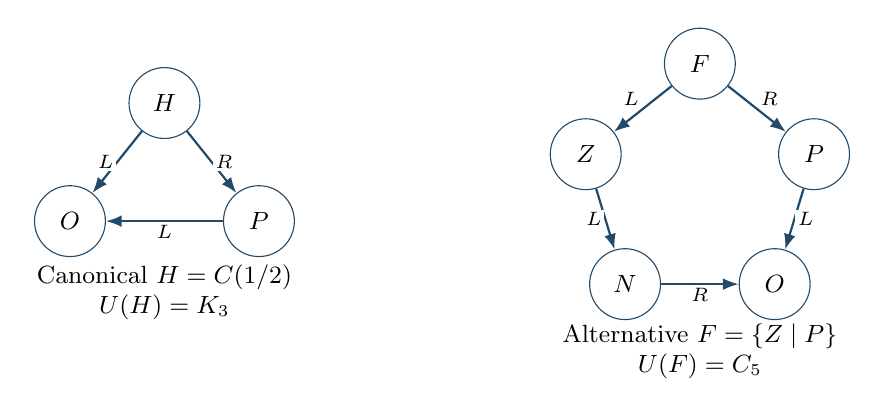
\begin{tikzpicture}[scale=1.0]
 \begin{scope}[xshift=-3.6cm]
  \node[vertex] (h) at (0,2.1) {$H$};
  \node[vertex] (p) at (1.2,0.6) {$P$};
  \node[vertex] (o) at (-1.2,0.6) {$O$};
  \draw[edge] (h)--node[elabel,left] {$L$}(o);
  \draw[edge] (h)--node[elabel,right] {$R$}(p);
  \draw[edge] (p)--node[elabel,below] {$L$}(o);
  \node[align=center,font=\small] at (0,-0.3)
   {Canonical $H=\can(1/2)$\\$U(H)=K_3$};
 \end{scope}
 \begin{scope}[xshift=3.2cm]
  \node[vertex] (f) at (0,2.6) {$F$};
  \node[vertex] (z) at (-1.45,1.45) {$Z$};
  \node[vertex] (n) at (-0.95,-0.2) {$N$};
  \node[vertex] (o) at (0.95,-0.2) {$O$};
  \node[vertex] (p) at (1.45,1.45) {$P$};
  \draw[edge] (f)--node[elabel,above left] {$L$}(z);
  \draw[edge] (z)--node[elabel,left] {$L$}(n);
  \draw[edge] (n)--node[elabel,below] {$R$}(o);
  \draw[edge] (f)--node[elabel,above right] {$R$}(p);
  \draw[edge] (p)--node[elabel,right] {$L$}(o);
  \node[align=center,font=\small] at (0,-1.05)
   {Alternative $F=\{Z\mid P\}$\\$U(F)=C_5$};
 \end{scope}
\end{tikzpicture}
\caption{The canonical triangle and the five-vertex obstruction. Vertex labels
name forms. In the right-hand graph $O$ and $Z$ both have value zero but are not
identical forms. Directions point from a form to an option.}
\label{fig:pentagon}
\end{figure}

The distinction is combinatorial rather than an artifact of edge directions or
numerical labels. No selection of three vertices in the alternative graph has
all three required edges. Also, the assertion is about ordinary, non-induced
subgraphs: permitting extra edges in a host would not help when the required
triangle is absent.

This counterexample does \emph{not} refute a minor version of the question. A
pentagon has a triangle as a minor and is a subdivision of a triangle. Keeping
these relations separate is essential when looking for a corrected statement.

\subsection{A second witness with no negative value}
\label{sec:second-witness}

The next theorem records an independently discovered witness. It is not a
relabelling of \cref{thm:pentagon}: what it buys is a counterexample whose
intermediate values are only $0$ and $1$, so that no negative number is imported
at all, and whose root has the empty form itself as a direct option.

\begin{theorem}[A second pentagon of value $1/2$]
\label{thm:second-pentagon}
The form $G$ in \eqref{eq:second-five} has value $1/2$, rank four, five vertices,
and five edges, and $U(G)=C_5$, drawn in \cref{fig:second-pentagon}. Hence
$U(\can(1/2))=K_3$ is not a subgraph of $U(G)$. The forms $F$ of \eqref{eq:main-five} and $G$ of \eqref{eq:second-five}
are distinct, and neither is the negation of the other.
\end{theorem}

\begin{proof}
The empty cut has value zero, so $\val(P)=1$: one is the simplest number
strictly above zero. Zero is the simplest number strictly below one, so
$\val(Z')=0$, and then $\val(P')=1$ by the same computation as for $P$. Finally
the simplest number strictly between $\val(O)=0$ and $\val(P')=1$ is $1/2$, so
$\val(G)=1/2$. Each cut is valid: the unary cuts impose no left-versus-right
comparison, and the final cut satisfies $0<1$.

The ranks of $O,P,Z',P',G$ are $0,1,2,3,4$, so all five forms are structurally
distinct even though two pairs share a value. The complete edge list is
\begin{equation}
\label{eq:second-edges}
 P\xrightarrow{\;L\;}O,\quad
 Z'\xrightarrow{\;R\;}P,\quad
 P'\xrightarrow{\;L\;}Z',\quad
 G\xrightarrow{\;L\;}O,\quad
 G\xrightarrow{\;R\;}P',
\end{equation}
and there are no others. Forgetting directions gives exactly the chordless
pentagon $G-O-P-Z'-P'-G$, which has no triangle.

For the last assertion, $F$ has rank three and $G$ rank four, so they are
distinct. The negation of $G$ has value $-1/2$, not $1/2$. More structurally,
$D(F)$ has a vertex of value $-1$ and $D(G)$ does not, and the root of $D(G)$ has
an edge to $O$ while the root of $D(F)$ does not.
\end{proof}

\begin{figure}[htbp]
\centering
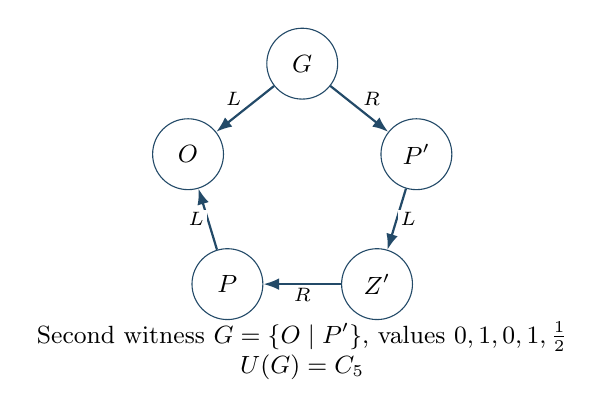
\begin{tikzpicture}[scale=1.0]
 \node[vertex] (g)  at (0,2.6) {$G$};
 \node[vertex] (o)  at (-1.45,1.45) {$O$};
 \node[vertex] (p)  at (-0.95,-0.2) {$P$};
 \node[vertex] (zp) at (0.95,-0.2) {$Z'$};
 \node[vertex] (pp) at (1.45,1.45) {$P'$};
 \draw[edge] (g)--node[elabel,above left] {$L$}(o);
 \draw[edge] (p)--node[elabel,left] {$L$}(o);
 \draw[edge] (zp)--node[elabel,below] {$R$}(p);
 \draw[edge] (pp)--node[elabel,right] {$L$}(zp);
 \draw[edge] (g)--node[elabel,above right] {$R$}(pp);
 \node[align=center,font=\small] at (0,-1.05)
  {Second witness $G=\{O\mid P'\}$, values $0,1,0,1,\tfrac12$\\$U(G)=C_5$};
\end{tikzpicture}
\caption{The second five-vertex counterexample. Here $O$ and $Z'$ are distinct
zero-valued forms and $P$ and $P'$ are distinct one-valued forms; no negative
value occurs. Compare \cref{fig:pentagon}, whose pentagon passes through a
vertex of value $-1$ and whose root is not adjacent to $O$.}
\label{fig:second-pentagon}
\end{figure}

\subsection{Exactly sixteen five-vertex counterexamples}

The two witnesses are not isolated, and they are not the only ones. The
exhaustive computation described in \cref{sec:verification} finds that among all
$3{,}860$ structurally distinct forms with at most five vertices there are
exactly sixteen whose underlying graph fails to contain its canonical underlying
graph, all of them at five vertices. Eight of the sixteen are triangle-free, and
four of those have value $1/2$. The form $F$ of \eqref{eq:main-five} is the
entry of rank three and girth five; the form $G$ of \eqref{eq:second-five} is a
different entry, of rank four and girth five. We do not claim either is unique.
The reconciliation of the two failure counts is discussed in
\cref{sec:verification}: the sixteen include girth-three forms of $\pm1/4$ and
$\pm3/4$, whose canonical graph is a diamond needing two triangles, and
restricting the sixteen to noninteger values of girth at least four returns
exactly the eight triangle-free forms.

\subsection{An independent order-theoretic verification}
\label{sec:comparison}

Neither conclusion depends on a heuristic reading of braces. For number forms the
recursive comparison relation can be written without any reference to rational
values:
\begin{equation}
\label{eq:comparison}
 X\leq Y
 \quad\Longleftrightarrow\quad
 \bigl(\forall X^{L}:\ \neg(Y\leq X^{L})\bigr)
 \ \wedge\
 \bigl(\forall Y^{R}:\ \neg(Y^{R}\leq X)\bigr).
\end{equation}
The accompanying checker implements \eqref{eq:comparison} using only option
identifiers, never cached rationals. Applied to the witnesses and to
$\can(1/2)$ it verifies both $F\leq\can(1/2)$ and $\can(1/2)\leq F$, both
$G\leq\can(1/2)$ and $\can(1/2)\leq G$, and the full comparison table of the six
forms involved against exact rational ordering. This is a structurally
different check from the second cut evaluator of \cref{sec:verification}, which
re-derives values but still works with numbers; \eqref{eq:comparison} never
computes a value at all. We use \eqref{eq:comparison} again as a proof tool in
\cref{sec:classification}.

\section{Canonical prefixes cannot disappear as values}
\label{sec:prefix}

The edges of a canonical representation are not unavoidable, but its simpler
prefix values are. We begin with the order-theoretic fact that makes this
precise.

\subsection{Sign expansions and convexity}

A surreal sign expansion is a sequence of $+$ and $-$ indexed by an ordinal.
The order is lexicographic, with an absent sign lying between $-$ and $+$. We
write $q\pref y$ when the sign expansion of $q$ is an initial segment of that
of $y$, allowing equality. Proper initial segments are simpler. These standard
facts and their relationship with cuts are developed in
\cite[Sections~2--3]{Berarducci2020}.

\begin{lemma}[Convexity of a simplicity cone]
\label[lemma]{lem:cone}
For any surreal $q$, the class
\begin{equation}
 I(q)=\{y:q\pref y\}
\end{equation}
is order-convex. In particular, if $q\pref y$ and $z$ lies between $q$ and $y$,
then $q\pref z$.
\end{lemma}

\begin{proof}
Suppose $a,c$ extend the sign expansion of $q$ and $a<z<c$. If $z$ fails to
extend $q$, let $\alpha$ be the first position before the end of $q$ at which
$z$ either terminates or differs from $q$. At that position $a$ and $c$ have
the same sign as $q$. Lexicographic comparison then places $z$ on the same
strict side of both $a$ and $c$, contradicting $a<z<c$.
\end{proof}

\begin{lemma}[Descent toward a prefix]
\label[lemma]{lem:descent}
Let $A$ be a numerical form, $y=\val(A)$, and $q\cpref y$.
If $q<y$, there is a left option $B$ with
\begin{equation}
 q\leq\val(B)<y,\qquad q\pref\val(B).
\end{equation}
If $y<q$, there is a right option $B$ with
\begin{equation}
 y<\val(B)\leq q,\qquad q\pref\val(B).
\end{equation}
\end{lemma}

\begin{proof}
The value $q$ cannot satisfy all the strict inequalities defining the cut of
$A$: if it did, $y$ would not be the simplest element of that interval, because
$q$ is a proper sign prefix of $y$. Suppose $q<y$. Every right-option value is
strictly greater than $y$, so no right option can exclude $q$. Some left option
must therefore have value at least $q$. Every left-option value is strictly less
than $y$, giving the required interval. Apply \cref{lem:cone}. The case $y<q$
is the left/right reversal.
\end{proof}

\begin{theorem}[Prefix occurrence]
\label{thm:prefix-occurrence}
If $A$ is a well-founded numerical form and $q\pref\val(A)$, then a descendant
subform of $A$ has value $q$. It can be reached by a finite directed path.
When $q<\val(A)$, the path can use only left-option edges; when
$q>\val(A)$, it can use only right-option edges.
\end{theorem}

\begin{proof}
Use induction on the well-founded rank of $A$. If $q=\val(A)$, the length-zero
path suffices. Otherwise \cref{lem:descent} supplies an option $B$ of smaller
rank with $q\pref\val(B)$. Apply the induction hypothesis to $B$ and prepend
the edge $A\to B$. In the case $q<\val(A)$ all subsequent values remain at
least $q$, so every nonterminal step uses a left option. The opposite case
uses right options throughout.
\end{proof}

The proof is deliberately a rank induction, not a compactness argument. It
works for arbitrary set-sized well-founded forms as well as finite ones. We
return to the transfinite case in \cref{sec:transfinite}.

\subsection{Finite prefixes and the canonical dependency graph}

For a finite value $x$, list its sign-prefix values by length:
\begin{equation}
\label{eq:prefix-list}
 p_0=0,p_1,\ldots,p_b=x,\qquad b=b(x).
\end{equation}
There is exactly one prefix at each length, although the values need not be
in increasing numerical order. For example, the prefixes of $5/8$ are
\begin{equation}
 0,\ 1,\ \tfrac12,\ \tfrac34,\ \tfrac58.
\end{equation}

\begin{lemma}[The finite canonical prefix chain]
\label[lemma]{lem:canonical-prefix}
Let $x\in\D$ and $k=\kappa(x)$. Then
\begin{equation}
\label{eq:birthday}
 b(x)=\lceil |x|\rceil+k.
\end{equation}
The vertices of $D(\can(x))$ are exactly $\can(p_0),\ldots,\can(p_b)$.
For each $j>0$, its options are the nearest earlier prefix below $p_j$ and the
nearest earlier prefix above $p_j$, omitting a side when no such prefix exists.
One of these options is $\can(p_{j-1})$. Exactly $k$ of $p_1,\ldots,p_b$ are
nonintegers.
\end{lemma}

\begin{proof}
For a positive integer $n$, the prefixes are $0,1,\ldots,n$, and the assertions
follow directly from \eqref{eq:dali}. Suppose $x$ is positive and nonintegral,
with $n<x<n+1$ and $n\geq0$. Its initial prefixes are $0,1,\ldots,n+1$.
Thereafter its prefixes are obtained by binary search in the interval $(n,n+1)$:
first test the midpoint, retain the half containing $x$, and repeat until the
midpoint is $x$.

At each step the current endpoints are precisely the nearest earlier prefix
values below and above the next midpoint. If that midpoint first occurs with
reduced denominator $2^r$, the endpoints are its two adjacent multiples on the
same $2^{-r}$ grid. Hence they are exactly the two options in
\eqref{eq:dali}, after reducing their fractions. One endpoint is the immediately
previous midpoint, except at the first midpoint, when the previous prefix is
$n+1$. Thus consecutive prefixes are linked by canonical option edges.

A reduced denominator $2^k$ is first reached on the $k$th midpoint step.
There are $n+1$ initial nonzero integer prefixes followed by $k$ noninteger
prefixes. This gives $b=n+1+k$, the vertex description, and all option claims.
Negation reverses the signs and exchanges option sides, proving the statements
for negative values. Zero is immediate.
\end{proof}

\begin{remark}[A second route to the birthday formula]
\label[remark]{rem:birthday-alt}
The identity \eqref{eq:birthday} alone, without the prefix-chain structure, also
follows by induction on $k$ directly from \eqref{eq:dali}, and the second route
is worth recording because it is what one needs when only the height of the
canonical form matters. Let $x\in(n,n+1)$ with $\kappa(x)=k$. For $k=1$ the two
canonical options are $\can(n)$ and $\can(n+1)$, of ranks $n$ and $n+1$, giving
$\rk(\can(x))=n+2$. For $k>1$, exactly one of the two neighbouring grid points
$(m\pm1)/2^k$ has reduced denominator exponent $k-1$, since exactly one of
$m-1,m+1$ has $2$-adic valuation one; the other has exponent at most $k-2$ or is
an integer. Both options stay in $[n,n+1]$, so by induction their ranks are at
most $n+k$ with the maximum $n+k$ attained, and $\rk(\can(x))=n+k+1$. Since
$b(x)=\rk(\can(x))$ and $\lceil x\rceil=n+1$, this is \eqref{eq:birthday}.
The same $2$-adic observation reappears in \cref{prop:fibonacci-alt}.
\end{remark}

\begin{theorem}[A path through every finite prefix]
\label{thm:prefix-path}
If $A$ is a finite form of value $x$ with prefixes \eqref{eq:prefix-list}, then
$D(A)$ contains a directed path on which the values
\begin{equation}
 p_b,p_{b-1},\ldots,p_0
\end{equation}
occur in that order. Additional vertices may occur between consecutive listed
values. In particular,
\begin{equation}
 \sizeV(A)\geq b(x)+1,\qquad \rk(A)\geq b(x).
\end{equation}
\end{theorem}

\begin{proof}
Starting at $A$, apply \cref{thm:prefix-occurrence} to $p_{b-1}$. From the
resulting form of value $p_{b-1}$, apply it to $p_{b-2}$, and continue. This is
a finite concatenation. Ranks strictly decrease along every edge, so the
concatenation cannot repeat a vertex. Each of the $b+1$ distinct prefix values
therefore appears on a single directed path, whose length is at least $b$.
\end{proof}

This is the basic positive replacement for literal subgraph containment. If
only reachability is required, the canonical prefix vertices can be represented
coherently in the finite case. The paths that realize different canonical edges
may overlap. The theorem consequently does not assert a topological-minor
embedding, for which appropriate internal vertex-disjointness would be needed.

\section{Sharp minima and an exact enumeration}
\label{sec:extrema}

\subsection{The denominator as minimum cycle rank}

\begin{lemma}[One-sided finite cuts have integer values]
\label[lemma]{lem:one-sided}
If a finite numerical form has a noninteger value, both its left and right
option sets are nonempty. In particular, it has at least two outgoing edges.
\end{lemma}

\begin{proof}
If both sets are empty, its value is zero. If only the left set is nonempty,
let $a$ be its largest option value. When $a<0$, zero is allowed and is simplest.
When $a\geq0$, the smallest integer strictly greater than $a$ is the simplest
surreal strictly greater than $a$. Thus the value is an integer. An empty left
set is handled by negation.
\end{proof}

\begin{theorem}[Exact graph minima]
\label{thm:minima}
Let $x\in\D$, $b=b(x)$, and $k=\kappa(x)$. Every finite form $A$ of value $x$
satisfies
\begin{equation}
\label{eq:minima}
 \sizeV(A)\geq b+1,\qquad
 \beta(A)\geq k,\qquad
 \sizeE(A)\geq b+k.
\end{equation}
The canonical form attains all three equalities simultaneously.
\end{theorem}

\begin{proof}
The vertex bound is \cref{thm:prefix-path}. Since $O$ is the unique sink,
\begin{align}
 \beta(A)
 &=\sum_{B\in V(D(A))}\outdeg(B)-\sizeV(A)+1 \notag\\
 &=\sum_{B\in V(D(A))\setminus\{O\}}
       \bigl(\outdeg(B)-1\bigr). \label{eq:beta-outdegree}
\end{align}
Every summand is nonnegative. By \cref{lem:canonical-prefix}, exactly $k$ of
the canonical prefix values are nonintegral. The prefix-occurrence theorem
provides distinct vertices with those values. Each has outdegree at least two
by \cref{lem:one-sided}, so these $k$ vertices contribute at least $k$ to
\eqref{eq:beta-outdegree}. This proves $\beta(A)\geq k$. Finally,
\begin{equation}
 \sizeE(A)=\sizeV(A)-1+\beta(A)\geq b+k.
\end{equation}

For the canonical form there are $b+1$ prefix vertices. Each of its $b-k$
nonzero integer vertices has one outgoing edge, and each of its $k$
noninteger vertices has two. Hence
\begin{equation}
 \sizeV(\can(x))=b+1,\qquad
 \sizeE(\can(x))=(b-k)+2k=b+k,\qquad
 \beta(\can(x))=k.
\end{equation}
\end{proof}

The cycle rank is the number of independent undirected cycles, not the number
of simple cycles and not the directed cycle count. Directed cycles never occur.
Thus the dyadic denominator has an exact representation-theoretic meaning:
its exponent is the least undirected cycle rank achievable by any finite form.

\begin{corollary}
\label[corollary]{cor:acyclic}
A finite surreal value has an acyclic underlying representation if and only if
it is an integer.
\end{corollary}
\begin{proof}
Integers have canonical path representations. A noninteger has $k\geq1$, so
every representation has positive cycle rank by \cref{thm:minima}.
\end{proof}

The next lemma reproves \cref{cor:acyclic} by a direct edge count that never
mentions prefixes, and it buys two things the first proof does not give: it
identifies the acyclic graph as a \emph{path}, and it isolates the unary
evaluation identities \eqref{eq:unary-integer}, which are used repeatedly in
\cref{sec:odd,sec:sparse}.

\begin{lemma}[Forest obstruction]
\label[lemma]{lem:forest}
If $A$ is finite and $U(A)$ is a forest, then $U(A)$ is a path and $\val(A)$ is
an integer. Moreover, for a form $Y$ of integer value $n$,
\begin{equation}
\label{eq:unary-integer}
 \val\bigl(\cut{Y}{}\bigr)=\max(0,n+1),
 \qquad
 \val\bigl(\cut{}{Y}\bigr)=\min(0,n-1).
\end{equation}
\end{lemma}

\begin{proof}
The graph is connected, so a forest here is a tree: with $\sizeV$ vertices it has
$\sizeV-1$ edges. Every vertex except the unique sink $O$ has at least one
outgoing edge, so the outdegree sum is at least $\sizeV-1$; equality forces every
form other than $O$ to have exactly one option. Since the root reaches every
vertex, the whole graph is a single directed path ending at $O$.

For \eqref{eq:unary-integer}, if $n<0$ then zero satisfies the cut $\cut{Y}{}$
and is simplest; if $n\geq0$ the simplest number strictly above $n$ is $n+1$. The
right-hand identity is the reflection. Starting from $\val(O)=0$ and proceeding
up the path, every value is an integer.
\end{proof}

\subsection{Classifying every vertex-minimal form}

\begin{theorem}[The vertex-minimal forms]
\label{thm:minimal-forms}
Fix $x\in\D$, with prefixes $p_0,\ldots,p_b$, and put $k=\kappa(x)$.
A finite form $A$ of value $x$ has exactly $b+1$ vertices if and only if it can
be built as follows. Use one vertex $A_j$ of value $p_j$ for each $0\leq j\leq b$,
with $A_0=O$. At each $A_j$, include the canonical nearest-prefix options.
Independently add or omit any other earlier-prefix option $A_i$ with $i<j$,
placing it on the left when $p_i<p_j$ and on the right when $p_i>p_j$.

Consequently every vertex-minimal form contains $D(\can(x))$ as a rooted,
value- and side-preserving spanning subgraph, and
\begin{equation}
\label{eq:count-minimal}
 \#\{A:\val(A)=x,\ \sizeV(A)=b+1\}
 =2^{\binom{b+1}{2}-(b+k)}
 =2^{b(b-1)/2-k}.
\end{equation}
\end{theorem}

\begin{proof}
Suppose first that $A$ has $b+1$ vertices. The path in
\cref{thm:prefix-path} already contains at least this many vertices. Therefore
it exhausts the graph and has no extra vertices between the prefixes. Denote
its vertices by $A_b,A_{b-1},\ldots,A_0$, where $\val(A_j)=p_j$. Every edge
must go from some $A_j$ to an earlier $A_i$: an edge in the reverse direction
would combine with the path to create a directed cycle.

Fix $j>0$. If there is an earlier prefix below $p_j$, let $\ell$ be the largest
such value. The vertex of value $\ell$ must be a left option of $A_j$. Otherwise
all actual left-option values are strictly below $\ell$, while all right-option
values are strictly above $p_j$ and hence above $\ell$. The simpler value
$\ell$ would then satisfy the cut of $A_j$, a contradiction. The smallest
earlier prefix above $p_j$, when present, is likewise a mandatory right option.
By \cref{lem:canonical-prefix}, these are precisely the canonical options.
Every other possible edge has its side determined by numerical comparison.

Conversely, perform the stated construction in increasing order of $j$.
Inductively, all earlier vertices have their assigned prefix values. The
mandatory nearest options already give the cut value $p_j$. Adding more
earlier prefixes on their permitted sides changes neither extreme bound, so it
does not change the value. All vertices are distinct because their values are
distinct. The consecutive-prefix edges are mandatory, so the root reaches
every vertex and the closure has exactly $b+1$ vertices.

There are $\binom{b+1}{2}$ possible edges from later to earlier prefixes, each
with a uniquely determined side. Of these, exactly $b+k$ are mandatory by
\cref{thm:minima}; every remaining edge is independently optional. Distinct
choices produce distinct forms: from the final form one recovers its uniquely
valued prefix vertices and all their edge choices. This proves the count and
the spanning statement.
\end{proof}

Notice what the theorem does \emph{not} say. The vertex $A_j$ need not be
literally identical to $\can(p_j)$, because it may have extra options. The
spanning embedding sends the canonical vertex of value $p_j$ to $A_j$.

\begin{corollary}[Unique edge-minimizer]
\label[corollary]{cor:edge-unique}
The canonical form $\can(x)$ is the unique finite form of value $x$ with
$\sizeE=b+k$.
\end{corollary}

\begin{proof}
Equality in the edge bound forces both $\sizeV=b+1$ and $\beta=k$. The
classification then permits no optional edges, because its mandatory edges
already number $b+k$. The recursive construction is therefore exactly
\eqref{eq:dali}.
\end{proof}

\begin{table}[htbp]
\centering
\begin{tabular}{@{}rccrrr@{}}
\toprule
Value $x$ & $b$ & $k$ & Minimum vertices & Minimum edges & Vertex-minimal forms\\
\midrule
$0$       &0&0&1&0&1\\
$1/2$     &2&1&3&3&1\\
$1/4$     &3&2&4&5&2\\
$3/4$     &3&2&4&5&2\\
$3/2$     &3&1&4&4&4\\
$3$       &3&0&4&3&8\\
$5/8$     &4&3&5&7&8\\
$5/2$     &4&1&5&5&32\\
$4$       &4&0&5&4&64\\
\bottomrule
\end{tabular}
\caption{The exact minima and enumeration. Negating a value gives the same
counts. The accompanying exhaustive computation checks all value classes with
$b\leq4$, including every row in this table.}
\label{tab:minimal}
\end{table}

\section{Sharp smallness and the failure of minimum rank}
\label{sec:smallness}

\subsection{Four vertices are never enough}

Both halves of this section, and also the exact extremal function of
\cref{sec:odd}, rest on one case analysis: the possible dependency orientations
of a quadrilateral. We isolate it once.

\begin{lemma}[Triangle-free forms on at most four vertices]
\label[lemma]{lem:quadrilateral}
Let $A$ be a finite form with at most four vertices whose underlying graph
$U(A)$ is triangle-free. Then $\val(A)$ is an integer. Equivalently, every
finite form of noninteger value on at most four vertices has a triangle in its
underlying graph.
\end{lemma}

\begin{proof}
If $U(A)$ has no cycle, \cref{lem:forest} gives an integer value. Otherwise
$U(A)$ is connected, triangle-free, has at most four vertices, and has a cycle,
so it is exactly $C_4$.

The dependency orientation of this quadrilateral has a unique source, namely the
root, and a unique sink, namely $O$. It therefore consists of two internally
disjoint directed root-to-$O$ paths whose lengths sum to four: either $(2,2)$ or
$(1,3)$. All their intermediate vertices are unary forms, so
\eqref{eq:unary-integer} evaluates them.

In the $(2,2)$ case the two intermediate forms are distinct unary forms over
$O$, namely $\can(-1)$ and $\can(1)$, of values $-1$ and $1$. If the root has
only one nonempty option side, its value is an integer by \cref{lem:one-sided}.
If both sides are nonempty, the only valid arrangement is
$\cut{\can(-1)}{\can(1)}$, of value zero.

In the $(1,3)$ case one root option is $O$ itself, and the other is a unary form
over a unary form over $O$, so by \eqref{eq:unary-integer} its value lies in
$\{-2,0,2\}$. A one-sided root again has integer value by
\cref{lem:one-sided}. If the two options lie on opposite sides, the value $0$ is
impossible, since a cut cannot have equal bounds on its two sides; the remaining
intervals are $(-2,0)$ and $(0,2)$, whose simplest elements are $-1$ and $1$.
Reversing which path is the long one is the same argument.

In every case the value is an integer.
\end{proof}

\begin{theorem}[Smallest size and rank of a counterexample]
\label{thm:smallest}
Every finite form with at most four vertices contains its canonical underlying
graph as an unlabelled undirected subgraph. Every finite form of rank at most
two has the same property. Hence the example in \cref{thm:pentagon} is smallest
both in vertex count and in form rank.
\end{theorem}

\begin{proof}
Let $A$ have $N\leq4$ vertices and value $x$. By \cref{thm:prefix-path},
$b(x)\leq N-1\leq3$. If $N=b(x)+1$, the spanning theorem
\ref{thm:minimal-forms} applies. If $x=n$ is an integer, the canonical graph
is a path of length $|n|$. The prefix-path theorem supplies a directed path
of at least that length in $D(A)$, so its undirected version contains the
required path.

The only remaining possibility is a noninteger of birthday at most two with
$N=4$: thus $x=1/2$ or $x=-1/2$. Its canonical graph is a triangle. By
\cref{lem:quadrilateral} a four-vertex form with a triangle-free graph has
integer value, so $U(A)$ has a triangle and the required embedding exists.

Finally, a form of rank at most two has no proper subforms other than $O$,
$\can(-1)$, and $\can(1)$. Its closure therefore has at most four vertices,
so the first part applies. The pentagon has five vertices and rank three.
\end{proof}

Note which hypotheses each half uses. \cref{lem:quadrilateral} is purely local:
it inspects four vertices and never mentions prefixes, and it is what supplies
the lower bound $m_{1/2}(4)\geq5$ in \cref{thm:extremal}. The rank half of
\cref{thm:smallest} and the four-vertex cases with $N=b(x)+1$ instead go through
the vertex-minimal spanning theorem, which \cref{lem:quadrilateral} alone cannot
reach: a four-vertex form of value $1/4$ has a triangle-containing graph, so the
lemma says nothing, whereas \cref{thm:minimal-forms} shows that its graph is the
canonical diamond.

This proof is independent of the exhaustive search. The computation in
\cref{sec:verification} supplies a separate audit of the small cases and produces
all sixteen counterexamples at five vertices.

\subsection{Least birthday is not enough}

It is tempting to rescue containment by requiring the representation to be born
as early as its value. That weaker size restriction does not work.

\begin{proposition}[A rank-minimal non-containing form]
\label[proposition]{prop:rank-minimal}
Let
\begin{equation}
\label{eq:quarter}
 O=\emptycut,\quad P=\cut{O}{},\quad
 Z'=\cut{}{P},\quad H=\cut{O}{P},\quad Q=\cut{Z'}{H}.
\end{equation}
Then $\val(Q)=1/4$ and $\rk(Q)=b(1/4)=3$, but
$U(\can(1/4))$ is not a subgraph of $U(Q)$.
\end{proposition}

\begin{proof}
The values of $Z'$ and $H$ are zero and $1/2$, so the value of $Q$ is $1/4$.
Their ranks are both two, giving $\rk(Q)=3$. The canonical quarter graph has
vertices $\can(1/4),H,P,O$ and edges
\begin{equation}
 \can(1/4)O,\quad\can(1/4)H,\quad HO,\quad HP,\quad PO.
\end{equation}
It is the diamond $K_4$ with one edge removed, and contains two distinct
triangles. The graph of $Q$ has edge set
\begin{equation}
 QZ',\quad QH,\quad Z'P,\quad HO,\quad HP,\quad PO.
\end{equation}
Its only triangle is $HPO$; the remaining cycle is the quadrilateral
$QZ'PHQ$. An injective subgraph map would send the two distinct triangles of
the diamond to two distinct triangles, which is impossible.
\end{proof}

\begin{figure}[htbp]
\centering
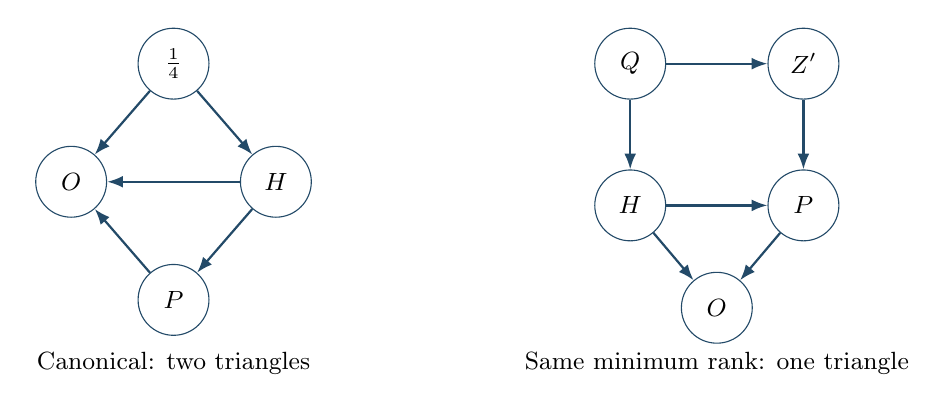
\begin{tikzpicture}
 \begin{scope}[xshift=-3.5cm]
  \node[vertex] (q) at (0,2.0) {$\frac14$};
  \node[vertex] (h) at (1.3,0.5) {$H$};
  \node[vertex] (o) at (-1.3,0.5) {$O$};
  \node[vertex] (p) at (0,-1.0) {$P$};
  \draw[edge] (q)--(h);\draw[edge] (q)--(o);
  \draw[edge] (h)--(o);\draw[edge] (h)--(p);\draw[edge] (p)--(o);
  \node[font=\small] at (0,-1.8) {Canonical: two triangles};
 \end{scope}
 \begin{scope}[xshift=3.4cm]
  \node[vertex] (q) at (-1.1,2.0) {$Q$};
  \node[vertex] (z) at (1.1,2.0) {$Z'$};
  \node[vertex] (h) at (-1.1,0.2) {$H$};
  \node[vertex] (p) at (1.1,0.2) {$P$};
  \node[vertex] (o) at (0,-1.1) {$O$};
  \draw[edge] (q)--(z);\draw[edge] (q)--(h);\draw[edge] (z)--(p);
  \draw[edge] (h)--(p);\draw[edge] (h)--(o);\draw[edge] (p)--(o);
  \node[font=\small] at (0,-1.8) {Same minimum rank: one triangle};
 \end{scope}
\end{tikzpicture}
\caption{Rank minimality does not force containment. Both roots have value
$1/4$ and rank three. Option-side labels are omitted; the defining cuts are
\eqref{eq:dali} and \eqref{eq:quarter}.}
\label{fig:quarter}
\end{figure}

Thus vertex minimality, rank minimality, and edge minimality are genuinely
different conditions. Vertex minimality permits many forms but forces the
canonical edges. Edge minimality forces the canonical form itself. Rank
minimality alone permits a counterexample.

\begin{remark}[A question answered]
\label[remark]{rem:cross-height}
\cref{prop:rank-minimal} settles, negatively, a question that the sparse side of
this investigation had left open: must every form whose rank equals the intrinsic
birthday of its value contain the canonical option graph of that value? The
pentagons of \cref{sec:pentagon} do not settle it, because $\rk(F)=3$ and
$\rk(G)=4$ while $b(1/2)=2$, so neither is rank-minimal. The form $Q$ is
rank-minimal and still fails containment, under the unlabelled convention. The
question remains genuinely open for other containment conventions, and the
transfinite example of \cref{prop:omega-highgirth} shows that at a limit
birthday the analogous unrestricted statement can fail for a different reason.
\end{remark}

\section{Cycle representations of one half, and exact optimality}
\label{sec:odd}

Each of the two pentagons extends to its own infinite family of cycles, and a
third family supplies the even lengths. Together they realize every cycle length
except four, and this is enough to determine the exact girth--size tradeoff at
the value $1/2$.

\subsection{First odd family: a zero spine through \texorpdfstring{$-1$}{-1}}

The rank-minimal pentagon extends to a particularly transparent infinite family.
Define a zero-valued spine by
\begin{equation}
\label{eq:zero-spine}
 Z_0=O,\qquad N_i=\cut{}{Z_i},\qquad
 Z_{i+1}=\cut{N_i}{}\qquad(i\geq0).
\end{equation}

\begin{lemma}
\label[lemma]{lem:zero-spine}
For every $i\geq0$,
\begin{equation}
 \val(Z_i)=0,\quad \rk(Z_i)=2i,\qquad
 \val(N_i)=-1,\quad \rk(N_i)=2i+1.
\end{equation}
The graph of $Z_i$ is a path of length $2i$, with alternating values $0,-1$.
All vertices on this path are structurally distinct.
\end{lemma}
\begin{proof}
Induct on $i$. A right-only cut bounded by zero has value $-1$; a left-only cut
bounded by $-1$ has value zero. Each construction raises rank by one. Distinct
ranks give distinct forms, and every noninitial spine vertex has exactly one
option, namely the preceding vertex of the path.
\end{proof}

\begin{theorem}[Odd-cycle family]
\label{thm:odd-cycle}
Let $P=\can(1)$ and, for $m\geq1$, set
\begin{equation}
 F_m=\cut{Z_m}{P}.
\end{equation}
Then
\begin{equation}
\label{eq:odd-stats}
 \val(F_m)=\tfrac12,\qquad
 \rk(F_m)=2m+1,\qquad
 U(F_m)=C_{2m+3},\qquad
 \beta(F_m)=1.
\end{equation}
\end{theorem}

\begin{proof}
The two root-option values are zero and one. The left root-to-$O$ path has
length $2m+1$, and the right path $F_m\to P\to O$ has length two. Their
internal vertices are disjoint, since the spine values are only zero and
$-1$, whereas $P$ has value one. The two paths therefore form a chordless
cycle of length $2m+3$. The rank is one more than that of $Z_m$, and a cycle
has cycle rank one.
\end{proof}

For $m=1$ this is $F_1=\cut{Z_1}{P}$, of rank three; it is the pentagon of
\eqref{eq:main-five}, since $Z_1=\cut{N_0}{}$ and $N_0=\cut{}{O}$.

This family shows that the least possible cycle rank does not imply a bound on
girth, even for the single fixed value $1/2$. It also supplies counterexamples
whose distance from the canonical local triangle can be made arbitrarily large
in the ordinary graph-theoretic sense of excluding every short cycle.

\subsection{Second odd family: an alternating \texorpdfstring{$0/1$}{0/1} spine}

The second witness generalizes along a different spine, on the other side of the
root, and through nonnegative values only. What this family buys is that it
contains the canonical triangle itself as its initial member, so the passage from
the canonical form to a counterexample happens inside one uniform construction.
Put $K_0=O$ and
\begin{equation}
\label{eq:alternating-spine}
 K_{j+1}=
 \begin{cases}
  \cut{K_j}{}, & j\text{ even},\\[2pt]
  \cut{}{K_j}, & j\text{ odd}.
 \end{cases}
\end{equation}

\begin{lemma}
\label[lemma]{lem:alternating-spine}
For every $j\geq0$ we have $\rk(K_j)=j$, and
$\val(K_{2r})=0$, $\val(K_{2r+1})=1$. The forms $K_0,\ldots,K_j$ are pairwise
distinct and span a path of length $j$.
\end{lemma}

\begin{proof}
Each step is a unary cut, so the rank increases by one and the new form has the
previous one as its only option; distinct ranks give distinct forms. The values
follow from \eqref{eq:unary-integer}: from value $0$ a left unary cut gives $1$,
and from value $1$ a right unary cut gives $0$.
\end{proof}

\begin{theorem}[Second odd-cycle family]
\label{thm:odd-cycle-two}
For $r\geq0$ put $G_r=\cut{K_0}{K_{2r+1}}$. Then
\begin{equation}
\label{eq:odd-two-stats}
 \val(G_r)=\tfrac12,\qquad
 \rk(G_r)=2r+2,\qquad
 U(G_r)=C_{2r+3},\qquad
 \beta(G_r)=1 .
\end{equation}
Here $G_0=\can(1/2)$ is the canonical triangle and $G_1=G$ is the second witness
\eqref{eq:second-five}.
\end{theorem}

\begin{proof}
The root options have values $0$ and $1$ by \cref{lem:alternating-spine}, so the
cut is valid and its value is $1/2$. Its graph is the path
$K_{2r+1}\to\cdots\to K_0$ of length $2r+1$ together with the two root edges to
its endpoints, giving a chordless cycle of length $2r+3$; no chord exists because
each $K_{j+1}$ has $K_j$ as its only option and the root's only options are
$K_0$ and $K_{2r+1}$. The rank is one more than $\rk(K_{2r+1})=2r+1$, and a
single cycle has cycle rank one. For $r=0$ the form is $\cut{O}{\can(1)}$, which
is \eqref{eq:dali} at $1/2$; for $r=1$ it is $\cut{O}{K_3}$ with
$K_3=P'$, which is \eqref{eq:second-five}.
\end{proof}

The two odd families are genuinely different constructions and neither subsumes
the other: they use different spine values ($0,-1$ against $0,1$), attach the
long arm to opposite sides of the root, and have different ranks at the same
cycle length, namely $2m+1$ against $2r+2$ for $C_{2m+3}=C_{2r+3}$. The first is
the rank-economical one; the second passes through the canonical form.

\subsection{An even family, and the full cycle spectrum}

Neither odd family gives an even cycle. A third construction does. Recall
$N_0=\cut{}{O}$, of value $-1$, from \eqref{eq:zero-spine}, and set
\begin{equation}
\label{eq:even-spine}
 N'=\cut{}{N_0},\qquad
 V_0=\cut{N'}{},\qquad
 V_{t+1}=\cut{}{\cut{V_t}{}}\qquad(t\geq0).
\end{equation}

\begin{theorem}[Even-cycle family]
\label{thm:even-cycle}
For every $t\geq0$ the form $V_t$ has value $0$ and rank $3+2t$, and the form
\begin{equation}
 G^{\mathrm{even}}_t=\cut{V_t}{P},\qquad P=\can(1),
\end{equation}
satisfies
\begin{equation}
\label{eq:even-stats}
 \val(G^{\mathrm{even}}_t)=\tfrac12,\qquad
 \rk(G^{\mathrm{even}}_t)=4+2t,\qquad
 U(G^{\mathrm{even}}_t)=C_{6+2t},\qquad
 \beta(G^{\mathrm{even}}_t)=1 .
\end{equation}
\end{theorem}

\begin{proof}
By \eqref{eq:unary-integer}, $\val(N')=-2$ and $\val(V_0)=0$, with ranks $2$ and
$3$. Inductively, $\cut{V_t}{}$ has value $1$ and rank $4+2t$, so $V_{t+1}$ has
value $0$ and rank $5+2t=3+2(t+1)$. All the forms on this branch are unary above
$N'$, hence pairwise distinct by rank, and the branch from $V_t$ down to $O$ is a
path with $3+2t$ edges.

The root cut has options of values $0$ and $1$, so $\val(G^{\mathrm{even}}_t)=1/2$.
The long branch and the short branch $P\to O$ meet only at $O$: the first form
above $O$ on the long branch is $N_0$, of value $-1$, not $P$, and every later
form on that branch has rank at least two while $\rk(P)=1$. The two internally
disjoint root-to-$O$ paths, of lengths $3+2t+1$ and $2$, therefore form a
chordless cycle of length $6+2t$.
\end{proof}

\begin{proposition}[All cycle lengths except four]
\label[proposition]{prop:allcycles}
For every integer $s=3$ or $s\geq5$ there is a finite form of value $1/2$ whose
underlying option graph is exactly $C_s$. The length $s=4$ is the unique
unattainable one: no form of value $1/2$, or indeed of any noninteger value, has
underlying graph $C_4$.
\end{proposition}

\begin{proof}
Odd lengths $s=2r+3\geq3$ come from \cref{thm:odd-cycle-two} and even lengths
$s=6+2t\geq6$ from \cref{thm:even-cycle}. A form whose graph is $C_4$ has four
vertices and no triangle, so \cref{lem:quadrilateral} makes its value an integer.
(Integers do realize $C_4$: the form $\cut{\can(-1)}{\can(1)}$ has value zero and
underlying graph $C_4$. The exclusion is of noninteger values, not of the graph
itself.)
\end{proof}

\subsection{The exact girth--size tradeoff at one half}

\begin{theorem}[Exact extremal function for $1/2$]
\label{thm:extremal}
For $g\geq3$ let
\begin{equation}
 m_{1/2}(g)=\min\bigl\{\sizeV(A):\val(A)=\tfrac12,\ \gir(U(A))\geq g\bigr\}.
\end{equation}
Then $m_{1/2}$ is given by \eqref{eq:overview-extremal}: it equals $3$ at $g=3$,
$5$ at $g=4$, and $g$ for every $g\geq5$. Moreover five vertices is the minimum
over all triangle-free finite representations of all noninteger values, and
$1/2$ attains that minimum.
\end{theorem}

\begin{proof}
By \cref{thm:minima} every representation of $1/2$ has $\beta\geq1$, so it
contains a cycle; if its girth is at least $g$ that cycle already uses at least
$g$ vertices, giving $m_{1/2}(g)\geq g$ for every $g$. For $g=3$ the canonical
triangle attains three. For $g\geq5$, \cref{prop:allcycles} supplies a form whose
whole graph is $C_g$, attaining $g$. For $g=4$ the bound $m_{1/2}(4)\geq4$ must
be improved: by \cref{lem:quadrilateral} a four-vertex triangle-free form has
integer value, so $m_{1/2}(4)\geq5$, and either pentagon of \cref{sec:pentagon}
attains five. The same lemma applies verbatim to every noninteger value, and the
half supplies a five-vertex triangle-free example.
\end{proof}

\begin{remark}[A question answered]
\label[remark]{rem:cross-girth}
\cref{thm:extremal} settles, for $x=1/2$, the optimal-girth-cost question raised
in \cref{q:girth-cost}: the least number of vertices at girth at least $g$ is
exactly $g$ once $g\geq5$, so the linear dependence of the general bound
\eqref{eq:output-bound} on $g$ is of the right order and has optimal constant
one at this value. Nothing here determines the constant for other noninteger
values.
\end{remark}

\begin{remark}
\label[remark]{rem:bipartite}
Even cycles of length at least six occur in \cref{thm:even-cycle}, so a bipartite
option graph need not represent an integer. The obstruction in
\cref{lem:forest} is the absence of \emph{all} cycles, not of odd cycles.
\end{remark}

\section{Arbitrarily large girth for every finite value}
\label{sec:high-girth}

The preceding construction treats one value. A uniform construction requires
more care: simply replacing repeated vertices by ``fresh copies'' is illegal
because identical forms are the same vertex. We first unfold the canonical
graph into an occurrence tree and then use different-rank zero forms to prevent
unwanted identifications.

\subsection{The occurrence tree and its zero leaves}

Assume $x>0$. Recursively unfold $D(\can(x))$ by giving every occurrence of an
option its own tree vertex, even when that form occurs elsewhere. This produces
a finite rooted occurrence tree $T_x$. It is an auxiliary tree, not yet a form
graph. Every leaf is an occurrence of $O$, and every internal vertex has
positive numerical value. Write
\begin{equation}
 I=\#\{\text{internal occurrences}\},\qquad
 L=\#\{\text{leaf occurrences}\}.
\end{equation}
Every root-to-leaf path has length at most $b=b(x)$.

Enumerate the leaves as $0,1,\ldots,L-1$ in any fixed order. Choose a positive
integer $M$ satisfying
\begin{equation}
\label{eq:spacing}
 2M>b.
\end{equation}
Replace leaf occurrence $i$ by the genuine form $Z_{Mi}$ from
\eqref{eq:zero-spine}. Rebuild all internal cuts, preserving their original
left/right choices. Denote the resulting root form by $A_{x,M}$.

\begin{theorem}[Spaced-spine construction]
\label{thm:high-girth}
For $x>0$ and $M$ satisfying \eqref{eq:spacing}, the form $A_{x,M}$ has value
$x$. Its dependency graph is exactly the occurrence tree with its distinct
leaves attached to the corresponding distinct vertices of the zero spine.
If $d_*$ is the depth in $T_x$ of the last leaf, then
\begin{align}
 \sizeV(A_{x,M})&=I+2M(L-1)+1,\label{eq:high-V}\\
 \sizeE(A_{x,M})&=I+L-1+2M(L-1),\label{eq:high-E}\\
 \beta(A_{x,M})&=L-1,\label{eq:high-beta}\\
 \rk(A_{x,M})&=2M(L-1)+d_* .\label{eq:high-rank}
\end{align}
The graph is acyclic if $L=1$; otherwise
\begin{equation}
\label{eq:high-girth}
 \gir(U(A_{x,M}))\geq2M+2.
\end{equation}
\end{theorem}

\begin{proof}
Every replacement leaf has value zero, the value of the leaf it replaces.
Induction upward through the finite occurrence tree therefore gives the
original value at every rebuilt internal vertex, including value $x$ at the
root. In particular, every rebuilt internal value is positive.

We now prove that no two distinct internal occurrences collapse to one form.
For an internal occurrence $v$ and a leaf $i$ below it, let $d(v,i)$ denote the
number of tree edges from $v$ to $i$. The recursive definition of rank gives
\begin{equation}
\label{eq:internal-rank}
 \rk(v)=\max_{i\text{ below }v}\bigl(2Mi+d(v,i)\bigr).
\end{equation}
Every distance in this formula is between one and $b$. Because $2M>b$, the
term with the largest leaf index $t(v)$ uniquely dominates all the others:
\begin{equation}
 \rk(v)=2Mt(v)+d(v,t(v)).
\end{equation}
If two internal occurrences have different largest leaf indices, their ranks
lie in disjoint intervals of length at most $b$, so the ranks differ. If they
have the same largest leaf index, both are ancestors of that one leaf and are
therefore comparable in the tree. Distinct ancestors have different distances
to the leaf, again giving different ranks. Thus all rebuilt internal vertices
are distinct forms.

No rebuilt internal vertex can equal any spine vertex, because internal values
are positive, whereas all spine values are zero or $-1$. The spine vertices
are mutually distinct by \cref{lem:zero-spine}. The chosen leaf attachment
points $Z_{Mi}$ are consequently distinct. This proves the asserted exact graph
structure, including the absence of hidden identifications.

The tree has $I+L$ vertices and $I+L-1$ edges. The spine from $Z_{M(L-1)}$ to
$O$ has $2M(L-1)+1$ vertices and $2M(L-1)$ edges. Identifying the $L$ leaves
with their attachment points gives \eqref{eq:high-V} and \eqref{eq:high-E}.
Subtracting yields \eqref{eq:high-beta}. Formula \eqref{eq:internal-rank} at
the root gives \eqref{eq:high-rank}.

Both the occurrence tree and the spine are individually acyclic. Any cycle in
their union must therefore include a nonempty spine segment. Choose a maximal
such segment within the cycle. Its endpoints must be distinct attachment
points: an interior spine vertex which is not an attachment has no edge leaving
the spine. Two attachment points are at spine distance at least $2M$. The
complementary part of the cycle has length at least two, since distinct leaves
of the occurrence tree are not joined by a tree edge. This proves the girth
bound. If there is only one leaf, there is only one attachment and no cycle.
\end{proof}

The rank-separation argument is the central technical precaution. It replaces
an unjustified appeal to labelled copies by an actual construction in the
hereditary syntax of surreal forms.

\begin{corollary}[Unbounded girth at every fixed value]
\label[corollary]{cor:unbounded-girth}
For every finite-birthday surreal value $x$ and every positive integer $g$, there exists
a finite form $A$ of value $x$ whose underlying graph has no cycle of length
less than $g$.
\end{corollary}
\begin{proof}
For positive $x$, take $M$ large enough that $2M>b(x)$ and $2M+2\geq g$.
For negative $x$, construct a form for $-x$ and negate it recursively, exchanging
left and right options. Negation is an involution on forms and induces an
isomorphism of underlying graphs. For zero, use $O$. We regard acyclic graphs
as having infinite girth.
\end{proof}

\begin{corollary}[Avoiding every fixed cyclic graph]
\label[corollary]{cor:avoid-graph}
Fix a finite-birthday surreal value $x$ and a finite graph $H$ containing a cycle. Some
finite representation of $x$ has no subgraph isomorphic to $H$.
\end{corollary}
\begin{proof}
Choose the representation in \cref{cor:unbounded-girth} with girth greater than
$|V(H)|$. Any copy of $H$ would contain a cycle of length at most $|V(H)|$.
\end{proof}

\subsection{Size bounds for the construction}

The construction is explicit, but unfolding can enlarge the canonical graph.
The number of leaves has a simple Fibonacci bound. Let
$f_1=f_2=1$ and $f_{r+2}=f_{r+1}+f_r$.

\begin{proposition}[A Fibonacci bound on the unfolded leaves]
\label[proposition]{prop:fibonacci}
If $x\in\D$ and $k=\kappa(x)$, the canonical occurrence tree has
\begin{equation}
 L\leq f_{k+2}.
\end{equation}
For each $k\geq0$, equality is attained by some value with denominator exponent
$k$. Moreover, $I\leq b(x)L$.
\end{proposition}

\begin{proof}
Every integer has a unary occurrence tree and hence one leaf. In any unit
interval, assign weight one to each integer endpoint. The number of leaves at
a dyadic midpoint is the sum of the leaf counts of its two endpoint forms.
Thus binary subdivision updates an endpoint-weight pair $(a,c)$ to either
$(a,a+c)$ or $(a+c,c)$, starting with $(1,1)$.

After $r$ updates, the larger endpoint weight is at most $f_{r+2}$ and the
smaller at most $f_{r+1}$. This follows by induction: the new larger weight is
the sum of the old pair, and the retained weight is at most the old larger one.
A value of reduced denominator $2^k$ is the midpoint after $k-1$ updates, so
its leaf count is at most $f_{k+2}$. At each update retain the larger of the
previous two weights. The successive sorted pairs are consecutive Fibonacci
numbers, proving attainability. The case $k=0$ is the integer case.

Finally, every internal occurrence lies on a path to some leaf, and each
root-to-leaf path contains at most $b(x)$ internal vertices. Counting
internal-vertex/descendant-leaf incidences yields $I\leq b(x)L$.
\end{proof}

The same bound has a second, shorter proof, which we record because it explains
the Fibonacci recursion arithmetically rather than through the geometry of
binary subdivision. It is stated for the binary cut tree $T(x)$ of
\cref{sec:sparse}, which is the tree obtained from $T_x$ by stopping at integer
leaves; the two trees have the same leaf count, because the unfolding below an
integer leaf is a unary chain and contributes exactly one $O$-leaf.

\begin{proposition}[A denominator-sensitive bound, second proof]
\label[proposition]{prop:fibonacci-alt}
If $x$ has reduced denominator $2^k$ with $k\geq1$, then $L\leq f_{k+2}$.
\end{proposition}

\begin{proof}
An integer contributes one leaf and a half-integer two, matching $f_2=1$ and
$f_3=2$. Let $x=m/2^k$ with $m$ odd and $k\geq2$. Of the two numerators $m-1$ and
$m+1$, exactly one has $2$-adic valuation one and the other has valuation at
least two, a zero numerator being read as an integer endpoint. Hence the two
canonical options have reduced denominator exponents exactly $k-1$ and at most
$k-2$. Their leaf counts add, so induction bounds the total by
$f_{k+1}+f_k=f_{k+2}$.
\end{proof}

This argument does not by itself establish attainment; the endpoint-weight
recursion in \cref{prop:fibonacci} does, for every $k$. The computations in
\cref{sec:verification} confirm attainment numerically for $k\leq8$, with
maximum leaf counts $2,3,5,8,13,21,34,55$, and separately over all denominator
exponents $0$ through $12$.

Combining the proposition with \eqref{eq:high-V} gives the concrete bound
\begin{equation}
\label{eq:output-bound}
 \sizeV(A_{x,M})
 \leq b(x)f_{k+2}+2M\bigl(f_{k+2}-1\bigr)+1.
\end{equation}
This is a graph-size bound, not a claim of optimality. The cycle rank produced
by the construction is $L-1$, which can exceed the minimum $k$. For example,
the canonical unfolding at $5/8$ has five leaves, so the construction has cycle
rank four, while the minimum possible cycle rank for that value is three.

\begin{table}[htbp]
\centering
\begin{tabular}{@{}rcrrrrrrr@{}}
\toprule
$x$ & $M$ & $L$ & $I$ & $\rk$ & $\sizeV$ & $\sizeE$ & $\beta$ & Girth\\
\midrule
$1/2$  &4&2&2&10&11&11&1&11\\
$3/4$  &4&3&4&18&21&22&2&11\\
$5/8$  &4&5&7&35&40&43&4&11\\
$5/16$ &4&8&10&60&67&73&7&11\\
$7/4$  &4&3&7&19&24&25&2&13\\
$-5/8$ &4&5&7&35&40&43&4&11\\
\bottomrule
\end{tabular}
\caption{Exact outputs of the spaced-spine implementation. The proved lower
bound for $M=4$ is girth at least ten; the actual girths in these examples are
larger. Leaves are enumerated by a left-before-right recursive traversal.}
\label{tab:high}
\end{table}

\section{A planar, degree-three construction: tree and spine}
\label{sec:sparse}

\cref{thm:high-girth} already gives arbitrarily large girth at every finite
value, with exact vertex, edge, cycle-rank, and rank formulas. This section
gives a second, independent route to large girth. It is not a variant of the
first: it unfolds a different tree, attaches it to a different spine, and proves
non-collapse by a different argument. What it buys is two graph properties the
spaced-spine construction cannot deliver --- its output is \emph{planar} and has
\emph{maximum degree at most three} --- at the price of losing the exact rank
formula \eqref{eq:high-rank} and of a size bound in different parameters, neither
bound implying the other.

The contrast between the two non-collapse proofs is the heart of the matter.
\cref{thm:high-girth} separates rebuilt vertices by \emph{rank arithmetic}: the
spacing condition $2M>b$ makes $\rk(v)=2Mt(v)+d(v,t(v))$ single out a dominant
leaf. The construction below separates them by \emph{value parity} --- internal
vertices are nonintegers, spine vertices are integers --- followed by a descent
through a singleton-option template. Neither argument can be substituted for the
other, and each is indispensable to its own construction: without it, the graph
argument would describe allocated objects rather than mathematical forms.

\subsection{Unfolding the canonical cut down to integers}

Let $x$ be a noninteger dyadic with $\kappa(x)=k$. Starting from
\eqref{eq:dali}, unfold every occurrence of a noninteger into its two canonical
options, but stop as soon as an integer is reached, and do not identify repeated
occurrences. The result is a finite ordered full binary tree $T(x)$.

Every internal vertex of $T(x)$ carries a noninteger dyadic label and every leaf
an integer label. If $x\in(n,n+1)$, every leaf label lies in $\{n,n+1\}$, since
the canonical options of a noninteger in $(n,n+1)$ stay in $[n,n+1]$. The
reduced denominator exponent strictly decreases along every internal edge, so
the tree is finite and its depth is at most $k$. Write $\ell=\ell(x)$ for the
number of leaves and enumerate them from left to right with integer labels
$n_1,\ldots,n_\ell$. A full binary tree with $\ell$ leaves has $\ell-1$ internal
vertices and $2\ell-2$ edges. For example,
\begin{equation}
 \tfrac58=\cut{\tfrac12}{\tfrac34},\qquad
 \tfrac34=\cut{\tfrac12}{1},\qquad
 \tfrac12=\cut{0}{1}
\end{equation}
unfolds to a tree with five leaves; at this stage the two occurrences of $1/2$
are separate subtrees. The leaf count obeys the same Fibonacci bound as before,
by \cref{prop:fibonacci} or \cref{prop:fibonacci-alt}.

\subsection{A unary spine with separated integer markers}

\begin{lemma}[Separated integer markers]
\label[lemma]{lem:markers}
Given integers $n_1,\ldots,n_\ell$ and an integer $d\geq1$, there is a unary
chain of pairwise distinct forms
\begin{equation}
 S_0=O,\quad S_1,\ldots,S_N,
\end{equation}
each $S_{i+1}$ having $S_i$ as its unique option, and marked indices
$0<s_1<\cdots<s_\ell=N$ such that
\begin{equation}
 \val(S_{s_j})=n_j,\qquad s_1\geq d,\qquad s_{j+1}-s_j\geq d .
\end{equation}
With $s_0=0$ it can be arranged that
\begin{equation}
\label{eq:gapbound}
 s_j-s_{j-1}\leq d+|n_j|+2 .
\end{equation}
Every spine form has rank equal to its index.
\end{lemma}

\begin{proof}
Each stage begins at the last constructed spine form, whose value is an integer.
If that value is positive, apply a unary right cut; if negative, a unary left
cut; \eqref{eq:unary-integer} shows that either resets the value to zero, and no
step is needed if the value is already zero.

From a zero-valued form, the two unary steps
\begin{equation}
 Y\longmapsto\cut{Y}{}\longmapsto\cut{}{\cut{Y}{}}
\end{equation}
return to value zero through value one, again by \eqref{eq:unary-integer}.
Repeat this pair $\lceil d/2\rceil$ times, which inserts between $d$ and $d+1$
edges. Finally take $|n_j|$ unary left steps from the resulting zero when
$n_j>0$, or $|n_j|$ unary right steps when $n_j<0$; the value reaches $n_j$.
Mark that index.

The stage uses at least $d$ edges and at most $1+(d+1)+|n_j|$, which is
\eqref{eq:gapbound}. Each new form has the previous one as its only option, so
its rank is one larger; distinct ranks make all spine forms distinct.
\end{proof}

\subsection{Substituting the markers}

Replace the $j$th integer leaf occurrence of $T(x)$ by the actual form
$S_{s_j}$, and rebuild every internal vertex as the singleton-left,
singleton-right cut with the same tree pattern as before. Call the resulting
root $X_{x,d}$.

\begin{lemma}[Value preservation]
\label[lemma]{lem:values}
Every rebuilt internal vertex is a valid numerical form whose value is its
original label in $T(x)$. In particular $\val(X_{x,d})=x$.
\end{lemma}

\begin{proof}
At the leaves the assertion is \cref{lem:markers}. At an internal vertex the two
rebuilt option values are exactly the two values of the corresponding canonical
cut, so they are strictly ordered and the simplest number between them is the
original label. Bottom-up induction gives validity and preserves every value.
\end{proof}

\begin{lemma}[No unintended identifications]
\label[lemma]{lem:nocollapse}
Distinct internal occurrences of $T(x)$ become distinct forms; none equals a
spine form; and distinct leaf occurrences are attached to distinct spine forms.
\end{lemma}

\begin{proof}
Spine forms have integer values, while by \cref{lem:values} every rebuilt
internal form has a noninteger value; so the two classes are disjoint. The
markers are distinct by \cref{lem:markers}.

Suppose two different internal occurrences became the same form. They would then
have the same value, say $r$, and the unfolded canonical template below an
occurrence labelled $r$ is determined by $r$ alone. Since each rebuilt left and
each rebuilt right option set is a singleton, equality of the two forms forces
equality of their left children, then of their right children, and inductively of
their corresponding descendants along every fixed left/right path in that
template. Follow one such path down to an integer leaf. The two occurrences then
force two corresponding markers to coincide. But every leaf occurrence of the
whole unfolded tree received a distinct marker, a contradiction.
\end{proof}

The lemma establishes the exact graph, not merely an upper bound for it:
$U(X_{x,d})$ consists of the spine path together with the binary tree $T(x)$,
whose $\ell$ leaves are attached to distinct marked spine vertices. No further
merging and no further edge is present.

\subsection{Girth, degree, and planarity}

\begin{lemma}[Graph bounds]
\label[lemma]{lem:graphbounds}
The graph $U(X_{x,d})$ is planar, has maximum degree at most three, and has
girth at least $d+2$.
\end{lemma}

\begin{proof}
Both the tree and the spine are acyclic, so a simple cycle in their union uses
edges of both kinds. On such a cycle take a maximal nonempty segment of spine
edges. Its endpoints are two different attachment vertices, because only those
have edges leaving the spine, and their indices differ by at least $d$; so the
segment has at least $d$ edges. The cycle also uses at least two tree edges, one
to leave the spine and one to return. Its length is therefore at least $d+2$.

For the degrees: an internal non-root tree vertex has two children and one
parent; the root has two children only; a marked spine vertex has at most two
spine neighbours and one tree parent; an unmarked spine vertex has at most two
neighbours. So every degree is at most three.

For planarity, draw the ordered binary tree with its leaves in left-to-right
order on a horizontal line and all other tree vertices above that line; such a
drawing exists recursively, by placing the two subtrees in disjoint horizontal
intervals. Join consecutive marked leaves by a path drawn below the line,
inserting the required unmarked spine vertices between them, and extend the
initial segment down to $S_0$ to the left. No crossings are introduced. The
markers were assigned in exactly this leaf order, so the drawing represents the
actual graph.
\end{proof}

\begin{theorem}[Planar high-girth representation theorem]
\label{thm:sparse}
For every dyadic $x$ and every integer $g\geq3$ there is a finite numerical form
$X$ with $\val(X)=x$ whose underlying option graph is planar, has maximum degree
at most three, and has girth at least $g$. A forest is assigned infinite girth.
\end{theorem}

\begin{proof}
If $x$ is an integer, take the canonical path $\can(x)$, which is acyclic and
has maximum degree at most two. Otherwise apply the construction with $d=g-2$
and use \cref{lem:values,lem:nocollapse,lem:graphbounds}.
\end{proof}

\subsection{Explicit size and height bounds}

Let $\ell=\ell(x)$, let $k=\kappa(x)$, and put $\mu=\max_j|n_j|$. Summing
\eqref{eq:gapbound} gives $N\leq\ell(d+\mu+2)$. There are $N+1$ spine vertices
and $\ell-1$ new internal vertices, so
\begin{equation}
\label{eq:sizebound}
 \sizeV(X_{x,d})=N+\ell\leq\ell(d+\mu+3),
\end{equation}
and, since a directed path traverses at most $k$ internal tree edges before
entering the spine and then at most $N$ spine edges,
\begin{equation}
\label{eq:heightbound}
 \rk(X_{x,d})\leq N+k\leq\ell(d+\mu+2)+k .
\end{equation}
The edge count is exact:
\begin{equation}
\label{eq:edgecount}
 \sizeE(X_{x,d})=N+2\ell-2,
 \qquad
 \beta(X_{x,d})=\sizeE-\sizeV+1=\ell-1 .
\end{equation}
Raising the required girth therefore lengthens the spine without increasing the
number of independent cycles. For a fixed $x$ both bounds are linear in the
requested girth.

These bounds are stated in $\ell$, $\mu$, and $d$, whereas \eqref{eq:high-V} and
\eqref{eq:output-bound} are stated in $I$, $L$, $b(x)$, and $M$; neither implies
the other, and the cycle rank $\ell-1$ here is the same quantity as $L-1$ there
only because the two trees have the same leaf count. Neither construction is
claimed to be minimal. For the single value $1/2$ the cycle constructions of
\cref{sec:odd} are far smaller, and \cref{thm:extremal} shows they are optimal.

\section{Which canonical graphs are unavoidable?}
\label{sec:classification}

The large-girth theorems answer much more than the single half-valued example.
We give the classification twice, under two containment conventions of different
strength, with two independent proofs of the positive half. Both negative halves
reduce to the same observation, which we isolate first.

\begin{lemma}[A triangle in every noninteger canonical graph]
\label[lemma]{lem:canonical-triangle}
If $x\in\D\setminus\Z$ then $U(\can(x))$ contains a triangle.
\end{lemma}

\begin{proof}
Suppose first that $\kappa(x)=1$, so $x=n+\tfrac12$ for an integer $n$. The two
canonical options are $\can(n)$ and $\can(n+1)$, and these adjacent integer
forms are joined by an edge: $\can(n+1)\to\can(n)$ when $n\geq0$, and
$\can(n)\to\can(n+1)$ when $n\leq-1$. With the root they form a triangle.

If $\kappa(x)=k>1$, one canonical option has denominator exponent exactly $k-1$
by \cref{rem:birthday-alt}. Following such options reaches a half-integer, whose
complete option graph occurs inside $D(\can(x))$, and the previous paragraph
supplies a triangle there.
\end{proof}

\subsection{The unlabelled classification}

\begin{theorem}[Exactly the integers, unlabelled version]
\label{thm:integer-classification}
For $x\in\D$, the graph $U(\can(x))$ is an unlabelled undirected subgraph of
every finite representation of $x$ if and only if $x\in\Z$.
\end{theorem}

\begin{proof}
If $x=n$ is an integer, $U(\can(n))$ is a path of length $|n|$. The path
provided by \cref{thm:prefix-path} has at least that many edges. Select a
subpath of the required length.

If $x$ is nonintegral, $U(\can(x))$ contains a triangle by
\cref{lem:canonical-triangle}. By \cref{cor:unbounded-girth}, or equally by
\cref{thm:sparse} with $g=4$, the value $x$ has a representation with no triangle
at all. Such a representation cannot contain $U(\can(x))$.
\end{proof}

The positive direction here uses unlabelled paths. It does not claim that
consecutive integer values always occur on consecutive option edges, or that
the integer classification extends unchanged to more restrictive kinds of
embedding. The negative direction is stronger: it already rules out the weakest
unlabelled notion.

\subsection{The rooted-colour classification}

The disclaimer just made is not the last word: the positive half does survive a
considerably stronger convention, by a different argument. Say that the
canonical option graph is \emph{rooted-colour unavoidable at value $x$} if every
finite form of value $x$ admits an injective embedding of $D(\can(x))$ which
preserves the root, the arrow directions, and the $L/R$ edge labels. Numerical
vertex labels are ignored, the subgraph need not be induced, and the image of the
canonical zero vertex is not required to be the sink of the ambient graph. This
demand is strictly stronger than the one in \cref{thm:integer-classification},
which forgets all four of root, direction, side, and value.

\begin{theorem}[Exactly the integers, rooted-colour version]
\label{thm:classification-rooted}
For $x\in\D$, the graph $D(\can(x))$ is rooted-colour unavoidable at value $x$ if
and only if $x\in\Z$. Moreover, for every noninteger $x$ there is a finite
representation of $x$ that excludes $U(\can(x))$ even as an unrooted,
unlabelled, undirected subgraph.
\end{theorem}

\begin{proof}
Let $x=n>0$ and let $A$ be any finite form of value $n$. For a nonnegative
integer $a$, comparison with $\can(a)$, which has no right options, gives
\begin{equation}
\label{eq:integer-comparison}
 \val(B)>a
 \quad\Longrightarrow\quad
 \text{some left option of }B\text{ has value at least }a .
\end{equation}
Indeed, if no left option of $B$ had value at least $a$, then
\eqref{eq:comparison} would give $B\leq\can(a)$, that is $\val(B)\leq a$.

Starting at the root, with value $n$, apply \eqref{eq:integer-comparison}
successively at the thresholds $n-1,n-2,\ldots,0$. This produces a directed path
of $n$ left-option edges from the root. Ranks strictly decrease along option
edges, so its vertices are distinct. The canonical graph of $n$ is exactly such a
path of $L$-edges rooted at its top, and mapping its successive vertices onto the
constructed path gives the required root-, direction-, and side-preserving
embedding. Reflection gives a path of right-option edges for a negative integer;
for zero the canonical graph is a single vertex.

If $x$ is noninteger, \cref{thm:sparse} with $g=4$ supplies a triangle-free
representation, while $U(\can(x))$ has a triangle by
\cref{lem:canonical-triangle}. So even the weakest containment fails, and a
fortiori the rooted-colour one does.
\end{proof}

\begin{remark}[Scope of the two positive halves]
The two proofs are independent and neither subsumes the other's method.
\cref{thm:integer-classification} routes through prefix occurrence, a
simplicity-theoretic fact about sign expansions; \cref{thm:classification-rooted}
routes through the recursive comparison \eqref{eq:comparison} and never mentions
sign expansions. What the second buys is the stronger conclusion: the embedded
path is rooted at the actual root and consists of genuine left-option edges in
the correct order. What neither asserts is that the embedded vertices carry the
canonical integer values, or that the canonical form occurs as a literal
subform. The negative halves have no such sensitivity: absence of a triangle
rules out every edge-preserving interpretation at once.
\end{remark}

\section{What happens at a transfinite birthday?}
\label{sec:transfinite}

The finite results already settle the selected question. The prefix argument,
however, also yields a useful observation about ordinal-indexed simplicity.
For an arbitrary set-sized well-founded form define
\begin{equation}
\label{eq:ordinal-rank}
 \rk(A)=\sup\{\rk(B)+1:B\in L_A\cup R_A\}.
\end{equation}
The supremum of the empty set is zero. At limit ranks this formula must not be
replaced by taking the supremum of the option ranks and then adding one.

\cref{thm:prefix-occurrence} was already proved for this ordinal rank. Thus
every sign prefix of a value occurs somewhere in every well-founded
representation. What can fail at a limit is the existence of one globally
coherent choice of representatives for all prefixes. The finite concatenation
in \cref{thm:prefix-path} does not justify a transfinite concatenation.

\begin{proposition}[A limit-stage coherence obstruction]
\label[proposition]{prop:omega}
There is a well-founded form of value $\omega$ and rank $\omega$ in which every
positive integer occurs as a subform value, but it is impossible to choose
vertices $B_n$ of value $n$, for all $n\geq1$, such that $B_{n+1}$ reaches $B_n$
for every $n$.
\end{proposition}

\begin{proof}
Use the zero spine \eqref{eq:zero-spine}. For $n\geq1$, define
\begin{equation}
 A_{n,0}=Z_n,\qquad
 A_{n,j+1}=\cut{A_{n,j}}{}\quad(0\leq j<n),
\end{equation}
and then put
\begin{equation}
 \Omega_* =\cut{A_{n,n}:n\geq1}{}.
\end{equation}
Induction gives
\begin{equation}
 \val(A_{n,j})=j,\qquad \rk(A_{n,j})=2n+j.
\end{equation}
The root cut is numerically the cut above all positive integers with no right
bound, so it has value $\omega$. Its rank is
\begin{equation}
 \rk(\Omega_*)=\sup_{n\geq1}(3n+1)=\omega.
\end{equation}

For $j>0$, positive vertices in different arms are distinct: equality of values
would force the same $j$, and equality of ranks would then force the same $n$.
A positive vertex in arm $n$ has a single outgoing edge to the preceding
vertex of that same arm. Once the path reaches its zero spine, it encounters
only zero and $-1$, never a positive vertex in another arm. Thus positive
vertices in distinct arms cannot reach one another.

Every vertex of value one belongs to a particular finite arm, say arm $n_0$.
The only positive finite-valued ancestors of that vertex are in the same arm
and have value at most $n_0$. A coherent sequence $B_n$ would make every $B_n$
reach $B_1$, including values larger than $n_0$, which is impossible. Each
individual integer nevertheless occurs in all sufficiently long arms.
\end{proof}

There is no conflict with well-foundedness. Every descending option path from
$\Omega_*$ first chooses a finite arm and then has finite length. The ordinal
rank is $\omega$ because these finite lengths are unbounded, not because one
infinite descending option path exists. Nor does the proposition contradict
prefix occurrence: it separates individual occurrence from a simultaneous
reachability-compatible selection.

\subsection{Large girth at a limit birthday costs nothing}

The second transfinite result concerns a different phenomenon and is logically
independent of \cref{prop:omega}: the first says that coherent prefix selection
can fail at a limit, the second says that sparsity can be achieved at a limit
without paying any birthday. Neither is used in the proof of the other.

Extend the canonical notation by
\begin{equation}
 \can(\omega)=\cut{\can(n):n\in\N}{},
\end{equation}
whose underlying graph is the infinite path of nonnegative integer forms together
with a root joined to every vertex; it contains triangles. For an integer
$d\geq1$ define instead
\begin{equation}
\label{eq:omega-form}
 W_d=\cut{\can(dn):n\in\N}{} .
\end{equation}
The options are a cofinal subsequence of the canonical integer forms, not new
copies of them.

\begin{proposition}[Exact high-girth forms of $\omega$]
\label[proposition]{prop:omega-highgirth}
For each $d\geq1$ the form $W_d$ has value $\omega$ and rank $\omega$. Its
underlying undirected option graph has girth exactly $d+2$, and every vertex
other than the root has degree at most three.
\end{proposition}

\begin{proof}
Every left option of $W_d$ is finite, so comparison with $\omega$, which has no
right options, gives $W_d\leq\omega$ by \eqref{eq:comparison}. Conversely $W_d$
exceeds each of its options $\can(dn)$, and those are unbounded in $\N$, so every
finite integer lies below $W_d$; applying \eqref{eq:comparison} in the other
direction gives $\omega\leq W_d$. Hence $\val(W_d)=\omega$.

For rank, \eqref{eq:ordinal-rank} gives
$\rk(W_d)=\sup_{n<\omega}(dn+1)=\omega$. Because the options are unbounded, their
descendants comprise every canonical finite integer form, so the underlying graph
is precisely the integer path together with a root joined at the vertices
$0,d,2d,\ldots$.

A simple cycle must pass through the root, since deleting the root leaves a path.
Such a cycle uses two distinct root attachments $di$ and $dj$, so its length is
$d|i-j|+2\geq d+2$, with equality for consecutive attachments. Finally, a
non-root vertex has its at most two path neighbours and at most one root edge.
\end{proof}

In particular $W_2$ is a triangle-free representation of $\omega$ whose rank is
$\omega$, the same as the birthday of its value and as the rank of
$\can(\omega)$. The finite pentagons raise the presentation rank above the
birthday of their value, but \cref{prop:omega-highgirth} shows that this cost is
not intrinsic to large girth: at a limit stage it vanishes. This is why the
finite minimum-rank question of \cref{rem:cross-height} does not have an
automatic transfinite analogue.

\subsection{Why the root's infinite degree is not an accident}

\cref{thm:sparse} bounds the maximum degree of its finite outputs by three, while
the root of $W_d$ has infinite degree. That asymmetry is forced.

\begin{proposition}[No transfinite form has finite outdegree everywhere]
\label[proposition]{prop:konig}
A well-founded form with only finitely many options at every descendant has
finite transitive option closure. Consequently every form of transfinite rank has
a vertex of infinite outdegree.
\end{proposition}

\begin{proof}
Suppose the closure were infinite. The root has finitely many options, so at
least one of them has infinite descendant closure; repeating the choice produces
an infinite sequence of successive options, contradicting well-foundedness. This
is the usual finite-branching argument behind K\"onig's lemma. A form with finite
transitive closure has finite rank.
\end{proof}

So the global degree bound of \cref{thm:sparse} provably cannot extend to a
representation of $\omega$; \cref{prop:omega-highgirth} confines the necessary
infinite degree to a single vertex, which is the best possible. No assertion is
made here about arbitrary surreals of ordinal birthday beyond these examples.

\section{Exact computation and reproducibility}
\label{sec:verification}

The proofs do not depend on experimental evidence. The accompanying program is
provided to make the finite examples inspectable, to check boundary cases, and
to detect implementation or transcription mistakes.

\subsection{Representation and arithmetic}

The implementation uses Python's standard library only. Each form is interned
by the ordered pair of its sorted left and right option-ID sets. Equal-valued
forms with different option sets remain distinct. All numerical values are
\code{fractions.Fraction} objects; there is no floating-point arithmetic.

To evaluate a finite cut, the main evaluator extracts its greatest left bound
and least right bound. It first checks whether zero is allowed, reflects an
entirely negative interval, and tests the least admissible positive integer.
When the interval contains no admissible integer, it searches successively
finer dyadic grids for the first admissible fraction. In an interval confined
between consecutive integers, the least denominator exponent gives the
simplest value. Explicitly, for a positive interval $(a,c)$ the least candidate
numerator at scale $2^r$ is
\begin{equation}
\label{eq:acceptance}
 p_r=\lfloor 2^r a\rfloor+1,
\end{equation}
which is accepted exactly when $p_r/2^r<c$; negative intervals are reflected.
Strict inequalities are used at every step, and no rounding tolerance or
floating-point comparison occurs anywhere.

Three separate oracles check the same objects in different ways, and all three
belong in the record because they fail differently.
\begin{enumerate}[label=(\roman*),leftmargin=2.2em]
\item \emph{A second cut evaluator.} For the exhaustive experiment, a separate
 evaluator enumerates values by intrinsic birthday and selects the first value
 satisfying every cut inequality. It does not use the main evaluator's
 dyadic-grid search \eqref{eq:acceptance}. The two evaluators agree on all
 $3{,}860$ forms encountered in the exhaustive closure.
\item \emph{A recursive comparison oracle.} A separate implementation of
 \eqref{eq:comparison} decides the order relation using only option
 identifiers, with no cached rationals at all. It verifies $F\leq\can(1/2)$,
 $\can(1/2)\leq F$, $G\leq\can(1/2)$, $\can(1/2)\leq G$ and the complete
 comparison table of the six forms involved against exact rational ordering.
 Unlike (i) it never computes a value, so it tests the order-theoretic content
 of the witnesses rather than the arithmetic kernel.
\item \emph{A graph oracle.} Girth is computed by breadth-first search from
 every vertex of the undirected adjacency structure built from option
 identifiers, and subgraph containment by the exact injective backtracking
 search described below. These are graph computations that use no arithmetic.
\end{enumerate}
Together these are independent algorithmic cross-checks, not an independent
formal verification of the entire software stack.

\subsection{Why the enumeration is exhaustive}

A finite dependency graph admits a topological ordering beginning with its
unique sink $O$ and ending with its root. For a fixed sequence of earlier
vertices, every possible new form is described by choosing, for each earlier
vertex, one of three states: absent, left option, or right option. The program
examines every such choice and rejects invalid cuts. It also rejects a new
vertex if that exact form has already appeared in the current sequence.

Some intermediate sequences contain vertices not used by the final root.
Therefore a root is recorded at size $n$ only when its transitive option closure
has exactly $n$ vertices. Different topological orderings of the same form are
deduplicated by structural interning: the $3{,}860$ distinct forms were obtained
from $4{,}651$ retained topological labellings. Conversely, every numerical form
of size at most the bound has at least one such ordering and is therefore
examined. This proves exhaustiveness for the stated finite vertex bound; it is
not a heuristic search restricted to unary or binary forms.

The implementation also checks ordinary, non-induced subgraph containment by
an exact injective backtracking search after forgetting directions, roots,
values, and option sides.

\begin{table}[htbp]
\centering
\begin{tabular}{@{}rrrrrr@{}}
\toprule
& & & \multicolumn{2}{c}{Triangle-free} & \\
\cmidrule(lr){4-5}
Vertices & Distinct forms & Noninteger & Noninteger & Value $1/2$
 & Canonical-subgraph failures\\
\midrule
1&1&0&0&0&0\\
2&2&0&0&0&0\\
3&10&2&0&0&0\\
4&123&32&0&0&0\\
5&3,724&1,200&8&4&16\\
\midrule
Total&3,860&1,234&8&4&16\\
\bottomrule
\end{tabular}
\caption{Complete enumeration through five vertices, by number of distinct
subforms, with structural identity rather than equality of values. These are not
counts by birthday. The last column tests the weakest unlabelled undirected
subgraph relation.}
\label{tab:enumeration}
\end{table}

\subsection{Reconciling the two failure statistics}

\cref{tab:enumeration} reports two different counts at five vertices, and both
are real. The sixteen canonical-subgraph failures are the outcome of the broader
test: they include girth-three forms of $1/4$, $3/4$, $-1/4$ and $-3/4$, which do
have a triangle but not the canonical diamond, whose embedding needs two
triangles sharing an edge. The eight triangle-free noninteger forms are the
outcome of the narrower test, which asks only for the absence of a triangle.
Filtering the sixteen certificates to those of noninteger value and girth at
least four returns exactly those eight, and four of the eight have value $1/2$
(the other four have value $-1/2$). So neither statistic implies the other:
the first is about failure of containment, the second about a specific local
pattern. Every noninteger canonical graph has a triangle by
\cref{lem:canonical-triangle}, which is why each of the eight is also one of the
sixteen.

The absence of a triangle-free noninteger form at four vertices is an
independent numerical confirmation of \cref{lem:quadrilateral}, and the four
half-valued optimal witnesses at five vertices confirm \cref{thm:extremal} at
$g=4$. The article prints two of the four; no uniqueness is claimed.

\subsection{Assertions that were actually run}

For every enumerated form, the program checks the prefix path, the birthday
lower bound, all three graph bounds, the value- and side-preserving spanning
statement whenever the vertex count is minimal, and uniqueness whenever the
edge count is minimal. It checks the enumeration formula in every one of the
$31$ value classes with birthday at most four. Exactly $31$ enumerated forms
attain the edge minimum, one canonical form for each class.

The infinite constructions are tested separately at twenty odd-cycle instances
($1\leq m\leq20$) and $126$ spaced-spine instances. The latter consist of all
$63$ values of birthday at most five, each at spacings $M=4$ and $M=6$. Each test
checks the value, rank, vertex count, edge count, cycle rank, and girth bound.
The Fibonacci leaf bound of \cref{prop:fibonacci} is checked at $4{,}096$
instances spanning denominator exponents $0$ through $12$, together with its
attainment claim. The experiment does not assert that a finite sample proves any
infinite family; those proofs are in
\cref{sec:odd,sec:high-girth,sec:sparse}.

The tree-and-spine construction of \cref{sec:sparse} has its own test suite,
which is kept separate because it exercises a different code path. It checks the
exact cycle family of \cref{sec:odd} at length three and at every length five
through sixty-four, giving $61$ certificates, and the sparse construction at
every value $x=p/32$ with $-64\leq p\leq64$ at requested girths $3,4,5,8,12$,
giving $645$ grid certificates. For every case it checks the value, the degree
bound, the girth, and a reconstructed certificate, and in the noninteger cases
also the vertex, edge, and height formulas \eqref{eq:sizebound}--\eqref{eq:edgecount}.
The largest grid graph had $176$ vertices and rank $166$. With the four showcase
examples of \cref{tab:showcase}, $710$ cycle or sparse-construction certificates
were generated and checked. Maximum leaf counts for denominator exponents one
through eight were measured as $2,3,5,8,13,21,34,55$, attaining the Fibonacci
bound in that range. Planarity is proved in \cref{lem:graphbounds}; it is not
separately software-tested.

\begin{table}[htbp]
\centering
\begin{tabular}{@{}rrrrrrrr@{}}
\toprule
Value & Requested & Actual & Leaves & Vertices & Edges & Rank & Size bound\\
 & girth & girth & & & & & \\
\midrule
$5/8$    &5 &7 &5 &30 &33 &27 &35\\
$-11/16$ &8 &9 &8 &66 &72 &61 &80\\
$53/32$  &12&15&13&176&187&166&195\\
$85/256$ &10&11&55&536&589&486&660\\
\bottomrule
\end{tabular}
\caption{Exact outputs of the tree-and-spine implementation of
\cref{sec:sparse}. The construction can exceed the requested girth, because the
reset and padding steps of \cref{lem:markers} add distance. The last column is
\eqref{eq:sizebound}.}
\label{tab:showcase}
\end{table}

The run bundled with this article used Python~3.13.5 and completed with every
assertion passing. The code targets Python~3.10 or newer and requires no
third-party packages. Do not use Python's \code{-O} flag, which disables
assertions and therefore disables most of the suite. From the archive's
top-level directory, run
\begin{lstlisting}
python3 code/verify.py
python3 code/verify_sparse.py
\end{lstlisting}
The first script's default vertex bound is five. A fresh output directory can be
selected with
\begin{lstlisting}
python3 code/verify.py --bound 5 --output fresh_results
\end{lstlisting}
A single bundled certificate can be rechecked directly:
\begin{lstlisting}
python3 -c "import json, sys; sys.path.insert(0, 'code'); \
 from verify_sparse import check_certificate; \
 check_certificate(json.load(open('examples/half_cycle_5.json'))); \
 print('Certificate passed')"
\end{lstlisting}
and a construction can be run interactively:
\begin{lstlisting}
from fractions import Fraction
from sparse_forms import sparse_form
arena, root, bounds = sparse_form(Fraction(5, 8), minimum_girth=5)
print(arena.metrics(root))
# {'value': '5/8', 'vertices': 30, 'edges': 33,
#  'height': 27, 'max_degree': 3, 'girth': 7}
arena.save(root, 'my_5_8_certificate.json')
\end{lstlisting}
In these outputs \code{height} is the form rank $\rk$ of this article, and
\code{girth: null} denotes an acyclic graph, that is, infinite girth.

\subsection{Artifacts and certificates}

The module \code{code/surreal\_forms.py} contains the exact form arena,
canonical construction, graph operations, the odd-cycle and spaced-spine
constructors, prefix-path extraction, and exhaustive enumeration. The script
\code{code/verify.py} performs the checks and writes the results. The directory
\code{results/} contains a machine-readable summary, CSV tables, the two named
counterexample certificates, and all sixteen small counterexamples. The module
\code{code/sparse\_forms.py} and the script \code{code/verify\_sparse.py} are
the second implementation: they contain the tree-and-spine constructor
\code{sparse\_form}, the full cycle spectrum, the recursive comparison oracle,
and the reusable \code{check\_certificate} routine, and they write to
\code{results/sparse\_*} and \code{examples/}.

Both implementations use the same certificate format, so certificates produced by
either can be rechecked by the other's reader. A certificate has a root
identifier and an array of node records in topological order. A typical record is
\begin{lstlisting}
{"id": 4, "left": [0], "right": [3], "value": "1/2", "height": 4}
\end{lstlisting}
All option identifiers in a record are strictly smaller than the record's own
identifier, which makes well-foundedness syntactically evident. Reconstruction
from the ordered pairs of option sets alone checks that each node is well
founded, is a valid numerical cut, and is structurally distinct from every
previously listed node, and that the root reaches every listed node. Values and
heights in the file are therefore recomputed, never trusted. A certificate also
carries the vertex and edge counts, maximum degree, rank, and girth; \code{null}
girth means an acyclic graph. Vertex identifiers are local names and are not part
of a form's identity.

The directory \code{examples/} holds eight certificates in this format, each with
a matching Graphviz \code{.dot} rendering of its option graph: the $C_3$, $C_5$,
$C_6$ and $C_{12}$ representations of $1/2$ from \cref{sec:odd} --- note that
\code{half\_cycle\_6} and \code{half\_cycle\_12} come from the even family
\eqref{eq:even-stats} --- and the four tree-and-spine outputs of
\cref{tab:showcase}. Graphviz is not a dependency of the tests or of the PDF
build; with it installed,
\code{dot -Tsvg examples/half\_cycle\_5.dot -o half\_cycle\_5.svg} renders one
optional standalone picture.

The two pentagon certificates are small enough to print. They are the five-row
tables in \cref{tab:certificate,tab:certificate-two}, and either one alone
suffices to verify the central counterexample by hand.

\begin{table}[htbp]
\centering
\begin{tabular}{@{}cllrr@{}}
\toprule
ID & Left-option IDs & Right-option IDs & Value & Rank\\
\midrule
0 & $\varnothing$ & $\varnothing$ & $0$ &0\\
1 & $\{0\}$ & $\varnothing$ & $1$ &1\\
2 & $\varnothing$ & $\{0\}$ & $-1$ &1\\
3 & $\{2\}$ & $\varnothing$ & $0$ &2\\
4 & $\{3\}$ & $\{1\}$ & $1/2$ &3\\
\bottomrule
\end{tabular}
\caption{A complete certificate for the first pentagon \eqref{eq:main-five}. The
root is vertex 4. This is entry $0$ of the sixteen five-vertex counterexamples.}
\label{tab:certificate}
\end{table}

\begin{table}[htbp]
\centering
\begin{tabular}{@{}cllrr@{}}
\toprule
ID & Left-option IDs & Right-option IDs & Value & Rank\\
\midrule
0 & $\varnothing$ & $\varnothing$ & $0$ &0\\
1 & $\{0\}$ & $\varnothing$ & $1$ &1\\
2 & $\varnothing$ & $\{1\}$ & $0$ &2\\
3 & $\{2\}$ & $\varnothing$ & $1$ &3\\
4 & $\{0\}$ & $\{3\}$ & $1/2$ &4\\
\bottomrule
\end{tabular}
\caption{A complete certificate for the second pentagon
\eqref{eq:second-five}. The root is vertex 4. Its undirected edge set is
$\{01,12,23,34,40\}$: every vertex has degree two and the graph is connected, so
it is $C_5$, while the canonical half has three mutually adjacent vertices. This
is entry $3$ of the same sixteen-element certified list, so the two witnesses are
demonstrably different members of one machine-checked enumeration.}
\label{tab:certificate-two}
\end{table}

\subsection{Limits of the computational evidence}

The rational evaluator and the certificate reconstruction share one simplicity
implementation within each of the two code bases. Between them they therefore
test serialization, extensionality, and internal consistency rather than
providing two entirely independent arithmetic kernels. The genuinely separate
checks are the ones that do not use the arithmetic at all: the recursive
comparison oracle \eqref{eq:comparison} and the breadth-first girth computation.
The second cut evaluator is separate in algorithm but not in language or
libraries. All the unbounded statements --- the all-dyadic girth theorems,
planarity, the extremal lower bound, the classifications, and the two $\omega$
propositions --- are established by the written proofs, not inferred from any
finite test set.

\section{Interpretation, limitations, and further questions}
\label{sec:discussion}

\subsection{What has been settled}

The literal canonical-subgraph assertion is false. Its failure is witnessed by
two extremely small numerical forms, not by a transfinite pathology or a
non-number game, and the exhaustive search shows those two are among exactly
sixteen five-vertex witnesses. The stronger large-girth theorems show that no
fixed finite cyclic graph can be forced inside every representation of a fixed
finite surreal value, and that the sparse representations can additionally be
taken planar of maximum degree three. For the single value $1/2$ the cost of
girth is known exactly. At the same time, the prefix theorem and the exact
minima reveal substantial rigidity that ordinary subgraph containment fails to
capture.

It is useful to separate three types of necessity. Prefix \emph{values} are
unavoidable. Certain amounts of graph \emph{complexity}, measured by vertex
count and cycle rank, are unavoidable. Individual canonical \emph{edges} are
unavoidable only under the additional vertex-minimality hypothesis proved
here. The distinction explains how a fixed dyadic denominator can force a
positive cycle rank while allowing all short cycles to be eliminated.

Recent work by Roughan studies the generation of random surreal forms for
benchmarking and emphasizes graph structure as a source of varied inputs
\cite{Roughan2025}. The constructions here provide deterministic complementary
test families: a fixed value with a prescribed long odd cycle, fixed values
with arbitrarily large girth, and complete sets of vertex-minimal forms.
These are mathematical input families, not measured claims about the running
time of an external implementation.

\subsection{A proof audit}

The logical dependencies are short and worth stating explicitly. The two
five-node counterexamples use only the evaluation of cuts with values $0$, $\pm1$
and $1/2$, structural identity, and the absence of a triangle in a pentagon;
their mathematical content can be checked without any general construction and
without any code.

The spaced-spine theorem \ref{thm:high-girth} uses the canonical occurrence
tree, the zero spine \eqref{eq:zero-spine}, the rank formula
\eqref{eq:internal-rank} with the spacing condition $2M>b$, and the observation
that a cycle in a tree joined to a path must traverse a spine segment between
attachment vertices. The tree-and-spine theorem \ref{thm:sparse} uses four
different facts: a finite canonical cut tree can be stopped at integer leaves;
unary cuts create distinct integer-valued markers arbitrarily far apart; replacing
an option by an equal-valued form preserves the value of a cut; and the same
cycle observation. In each construction the non-collapse lemma ---
the rank separation inside the proof of \cref{thm:high-girth}, and
\cref{lem:nocollapse} respectively --- is indispensable: without it the graph
argument would describe allocated objects rather than mathematical forms.

The classifications use the girth theorems only in the negative direction.
\cref{thm:integer-classification} obtains its positive half from prefix
occurrence; \cref{thm:classification-rooted} obtains its stronger positive half
from recursive comparison alone. The exact extremal function \ref{thm:extremal}
uses the two odd families, the even family, the forest obstruction, and the
complete four-vertex analysis \ref{lem:quadrilateral}. The two $\omega$ results
are independent of each other and of the finite constructions. None of these
arguments uses a conjectural estimate, a numerical approximation, or an
extrapolation from the finite enumeration.

\subsection{What has not been claimed}

The original source and the later benchmarking paper were inspected, together
with sign-expansion and Dali references. The target question was read in the 2018
arXiv version, at the caption of Figure~3 on printed page~7. A 2023 journal
version of the same paper is indexed in \emph{Mathematics Magazine} \textbf{96},
pages 329--343 \cite{Roughan2023}; its full text was not retrievable in this
research session, so the quoted wording is attributed to the accessible preprint
and is not asserted to occur unchanged in the journal version, nor is it asserted
that the journal version contains no answer. Searches for the canonical-subgraph
question, counterexamples, and girth constructions did not locate an earlier
resolution on 20 September 2026. Search coverage and publisher access were
limited. This supports treating the documented question as a research target,
but it does not certify the novelty of every theorem or exclude an answer in an
unindexed source or private correspondence. The prefix argument is a direct
application of standard simplicity and is presented with its proof, rather than
advertised as a new foundational principle.

No Lean or other proof-assistant formalization is included. The exhaustive
program checks a finite universe and explicit finite instances. The ordinal
arguments, the classifications, and the infinite families are justified by the
written mathematical proofs. None of the results is a theorem about all
combinatorial games: the numerical-cut condition is used essentially.

\subsection{Two questions answered along the way}

Two questions that each half of this investigation had left open are settled by
the other half, and we record the resolutions rather than reprinting the
questions as open.

First, whether a representation whose rank equals the intrinsic birthday of its
value must contain the canonical option graph: \cref{prop:rank-minimal} answers
this negatively at $x=1/4$, under the unlabelled convention, by a rank-minimal
form whose graph has one triangle where the canonical diamond needs two. See
\cref{rem:cross-height}. Second, the optimal girth cost at a fixed value:
\cref{thm:extremal} determines it exactly for $x=1/2$, where the answer is $g$
vertices for every $g\geq5$. See \cref{rem:cross-girth}. Both questions remain
open in the generality in which they were originally posed --- for other
containment conventions in the first case, and for other values in the second.

\subsection{Five questions left by this analysis}

\begin{question}[Cycle rank versus girth]
\label[question]{q:rank-girth}
For every dyadic $x$ with $\kappa(x)=k$, can arbitrarily large girth be achieved
while keeping $\beta=k$?
\end{question}
The answer is yes for integers and for $x=\pm1/2$ by the explicit path and
odd-cycle constructions. Neither uniform construction answers the question in
general: the spaced-spine construction has cycle rank $L-1$ and the
tree-and-spine construction has cycle rank $\ell-1$, and both may exceed $k$.
This is a natural question arising from the present proofs, not a claim that
its status has been exhaustively surveyed.

\begin{question}[Minor and subdivision replacements]
\label[question]{q:minors}
Which canonical dependency graphs are forced as undirected minors or
topological minors of every equivalent finite form?
\end{question}
Large girth alone is not an obstruction to either kind of containment. The
prefix-path theorem supplies overlapping reachability witnesses, not the
branch-set or disjoint-path conditions needed for these stronger conclusions.

\begin{question}[Optimal girth cost]
\label[question]{q:girth-cost}
For a fixed noninteger dyadic $x$, what is the least number of vertices needed
for a representation with girth at least $g$? Can the bound
\eqref{eq:output-bound} be improved uniformly in the denominator exponent?
\end{question}
For $1/2$, \cref{thm:extremal} gives the exact answer $g$ for $g\geq5$. For
general $x$, both proofs give a bound linear in $g$ with an explicit
value-dependent constant, since $M$ may be chosen proportional to $g+b(x)$ and
$d$ equals $g-2$. The Fibonacci estimate quantifies those constants but does not
establish an optimal dependence on $k$.

\begin{question}[Optimal sparse complexity, height included]
\label[question]{q:sparse-complexity}
For a fixed noninteger dyadic $x$, determine also the least form rank achievable
subject to girth at least $g$.
\end{question}
This is the companion of \cref{q:girth-cost} in the second size parameter.
\cref{thm:extremal} settles the vertex count for $x=1/2$ and says nothing about
rank; \eqref{eq:high-rank} and \eqref{eq:heightbound} give upper bounds only, and
the two constructions disagree about which is smaller.

\begin{question}[Restricted arithmetic presentations]
\label[question]{q:arithmetic}
Which canonical subgraphs are forced if the alternative forms are required to be
outputs of a specified collection of raw arithmetic operations on canonical
inputs, rather than arbitrary valid cuts?
\end{question}
Both witnesses here are valid cut constructions, and nothing in either proof
identifies them as outputs of any particular restricted arithmetic syntax. Such
a restriction would define a different problem, and it is the one direction in
this list that changes the class of admissible representations rather than the
notion of containment or the size measure.

\section{Conclusion}

A representation of $1/2$ need not contain its canonical triangle: the five
forms in \eqref{eq:main-five} instead form a pentagon, and so, differently, do
the five forms in \eqref{eq:second-five}. This gives a direct, fully finite
negative answer to the selected published question, twice over. The answer can
be strengthened in two complementary directions. On the flexible side,
representations of every finite value can avoid all cycles below an arbitrary
length, and can be taken planar with maximum degree three; at $1/2$ the exact
price of girth $g$ is $g$ vertices. On the rigid side, canonical prefix values
cannot disappear, and the least vertex count, edge count, and cycle rank are
exactly calculable from the birthday and denominator.

The sharp replacement for universal edge containment is therefore not that
canonical structure vanishes, but that it survives in a different form:
as prefix reachability, as minimum graph complexity, and as a mandatory
spanning graph precisely at minimum vertex size. The transfinite example shows
why even the reachability formulation must be handled carefully at limit
birthdays.

\appendix
\section{Verification pseudocode}
\label{app:pseudocode}

The exhaustive search is summarized below. \code{intern} identifies only
structurally equal forms. The actual implementation includes strict numerical
validity checks, exact values, ranks, and deduplication of recorded roots.

\begin{lstlisting}
search(prefix):
    root = last(prefix)
    if option_closure(root) contains every vertex of prefix:
        record root at size len(prefix)
    if len(prefix) == vertex_bound:
        return
    for choice in {absent, left, right} ^ len(prefix):
        L, R = option_sets(prefix, choice)
        if every value in L is strictly below every value in R:
            new = intern(L, R)
            if new not in prefix:
                search(prefix followed by new)

search([empty_form])
\end{lstlisting}

The finite prefix-path procedure is constructive as well. It uses exact
comparisons and the fact proved in \cref{lem:descent} that an eligible option
must exist.

\begin{lstlisting}
path = [root]
current = root
for q in proper_sign_prefixes(value(root)), longest first:
    while value(current) != q:
        if q < value(current):
            choose a left option B with q <= value(B) < value(current)
        else:
            choose a right option B with value(current) < value(B) <= q
        append B to path
        current = B
return path
\end{lstlisting}

In a finite graph, ranks strictly decrease and ensure termination. In the
transfinite proof, ordinal rank induction replaces any proposed numerical
iteration bound. The code implements only the finite algorithm.

\section{The tree-and-spine construction in pseudocode}
\label{app:sparse-pseudocode}

The following summarizes the mathematical construction of \cref{sec:sparse}. It
is not the code used as evidence; the executable implementation is
\code{code/sparse\_forms.py}.

\begin{lstlisting}
SPARSE(x, g):
    require x dyadic and g >= 3
    if x is an integer:
        return the canonical unary chain for x

    T := unfolded canonical binary cut tree for x,
         stopping each branch at its first integer
    d := g - 2
    spine := [empty form]
    markers := []

    for each integer leaf label n of T, in left-to-right order:
        reset the current integer value to 0 if necessary
        repeat ceil(d/2) times:
            append a unary left cut    # value 0 -> 1
            append a unary right cut   # value 1 -> 0
        append abs(n) unary cuts toward the integer n
        record the current form as this leaf's marker

    rebuild every internal node of T as {left_child | right_child}
    return the rebuilt root, interning by complete option sets
\end{lstlisting}

The reset and padding steps are what make the actual girth of the output exceed
the requested girth in \cref{tab:showcase}. Interning by complete option sets,
rather than by value or by allocation, is what \cref{lem:nocollapse} justifies.

\begin{thebibliography}{9}
\bibitem{Berarducci2020}
Alessandro Berarducci.
\newblock \emph{Surreal numbers, exponentiation and derivations}.
\newblock arXiv:2008.06878, 2020.
\newblock Sections 2--3 discuss sign expansions, simplicity, convexity, and cuts.
\newblock \url{https://arxiv.org/abs/2008.06878}.

\bibitem{Roughan2018}
Matthew Roughan.
\newblock \emph{Surreal Birthdays and Their Arithmetic}.
\newblock arXiv:1810.10373v2, 25 October 2018.
\newblock The subgraph question is in the caption to Figure 3, p.~7.
\newblock \url{https://arxiv.org/abs/1810.10373}.

\bibitem{Roughan2023}
Matthew Roughan.
\newblock \emph{Surreal Birthdays and Their Arithmetic}.
\newblock Mathematics Magazine \textbf{96} (2023), 329--343.
\newblock \href{https://doi.org/10.1080/0025570X.2023.2205819}
 {doi:10.1080/0025570X.2023.2205819}.
\newblock Bibliographic metadata located; the publisher's full text was not
retrieved in this research session, and no claim is made that the 2018 wording
persists unchanged in this version.

\bibitem{Roughan2025}
Matthew Roughan.
\newblock \emph{Evolutionary Generation of Random Surreal Numbers for Benchmarking}.
\newblock arXiv:2504.07152v1, 9 April 2025; GECCO '25 Companion.
\newblock \url{https://arxiv.org/abs/2504.07152}.

\bibitem{SchleicherStoll}
Dierk Schleicher and Michael Stoll.
\newblock \emph{An Introduction to Conway's Games and Numbers}.
\newblock arXiv:math/0410026v2, 30 September 2005.
\newblock Section 5.1 treats the simplicity theorem.
\newblock \url{https://arxiv.org/abs/math/0410026v2}.

\bibitem{Tondering2019}
Claus T{\o}ndering.
\newblock \emph{Surreal Numbers---An Introduction}.
\newblock Version 1.7, 31 January 2019.
\newblock The Dali construction is Eq.~(2.71), p.~25.
\newblock \url{https://www.tondering.dk/download/sur16.pdf}.
\newblock The file served at this URL identifies itself as version 1.7,
notwithstanding the filename.
\end{thebibliography}


\end{document}
